%%%%%%%%%%%%%%%%%%%%%%%%%%%%%%%%%%%%%%%%%%%%%%%%%%%%%%%%%%%%%%%%%%%%%%%%%%%%%
%%
%% Classes disponibles :
%%	- times : utilisation de la police Times par défaut.
%%	- these, sujthese, projthese, memoire, essai, rapport : pour
%%		générer la page de garde en fonction du type document.
%%	- french, english : selon la langue dans laquelle doit
%%		être rédigé le document.
%%  - ieee, apa : style des références bibliographiques
%%  - twoside : alternance des marges pour impression recto/verso
%%    vous devez décommenter la ligne 22 si vous utilisez cette classe
%%
%%%%%%%%%%%%%%%%%%%%%%%%%%%%%%%%%%%%%%%%%%%%%%%%%%%%%%%%%%%%%%%%%%%%%%%%%%%%%%
\documentclass[12pt,times,rapport,french,apa]{uqac}

%%%%%%%%%%%%%%%%%%%%%%%%%%%%%%%%%%%%%%%%%%%%%%%%%%%%%%%
%%
%% Décommenter la ligne suivante avec l'utilisation de
%% la classe "twoside"
%%
%%%%%%%%%%%%%%%%%%%%%%%%%%%%%%%%%%%%%%%%%%%%%%%%%%%%%%%
% \raggedbottom

%%%%%%%%%%%%%%%%%%%%%%%%%%%%%%%%%%%%%
%%
%% Préciser l'emplacement du fichier
%% contenant les acronymes.
%%
%%%%%%%%%%%%%%%%%%%%%%%%%%%%%%%%%%%%%
\acrolistpath{assets/acro}

%%%%%%%%%%%%%%%%%%%%%%%%%%%%%%%%%%%%%%%%%%%%%%%%%%%%%%%%
%%
%% Toutes les images utilisées doivent se trouver dans
%% le répertoire "assets/figure".
%%
%%%%%%%%%%%%%%%%%%%%%%%%%%%%%%%%%%%%%%%%%%%%%%%%%%%%%%%%
\graphicspath{{assets/figures/}}

%%%%%%%%%%%%%%%%%%%%%%%%%%%%%%%%%%%%
%%
%% Packages utilisateurs ci-dessous:
%%
%%%%%%%%%%%%%%%%%%%%%%%%%%%%%%%%%%%%
\usepackage{color, xcolor, soulutf8}
\usepackage{tikz}
\usetikzlibrary{babel}
\usepackage{chemfig}
\usepackage{chemnum}
\usepackage[europeanresistors,americaninductors]{circuitikz}
\usepackage{tikz-feynman}
\usepackage{hyperref}
\hypersetup{
  colorlinks=true,
  linkcolor=black,
  urlcolor=[rgb]{0,0.501,0.674},
  breaklinks=true,
  citecolor=[rgb]{0,0.501,0.674},
  bookmarks=true
}

\usepackage{listings}
\usepackage{xcolor}

\lstdefinestyle{bashstyle}{
  basicstyle=\ttfamily\small,   % smaller monospace
  breaklines=true,              % wrap long lines
  breakatwhitespace=false,      % allow breaking inside long URLs
  columns=fullflexible,
  keepspaces=true,              % keep alignment
  postbreak=\mbox{\textcolor{gray}{\(\hookrightarrow\)}\space} % wrap marker
}

%%%%%%%%%%%%%%%%%%%%%
%%
%% Césures manuelles
%%
%%%%%%%%%%%%%%%%%%%%%
% \hyphenation{con-nection con-nue con-cep-tion}

%%%%%%%%%%%%%%%%%%%%%%%%%%%%%%%%
%%
%% Gestion des lignes orphelines
%%
%%%%%%%%%%%%%%%%%%%%%%%%%%%%%%%%
\widowpenalty10000
\clubpenalty10000

\begin{document}
\pagestyle{empty}
\thispagestyle{empty}

%%%%%%%%%%%%%%%%%%%%%%%%%%%%%
%%
%% Titre, auteur et programme
%%
%%%%%%%%%%%%%%%%%%%%%%%%%%%%%

\title{Système de détection d'anomalies et de gestion de logs pour la sécurité des réseaux}
\author{Larzul Julien, Ian Bertrand, Tom Humeau, Alexis Georges}
\programme{Informatique}

%%%%%%%%%%%%%%%%%%%%%%%%%%%%%%%%%%%%%
%%
%% S’il y a lieu, indiquer le profil
%% ou la concentration du programme
%%
%%%%%%%%%%%%%%%%%%%%%%%%%%%%%%%%%%%%%
%\concentration{profil recherche}

%%%%%%%%%%%%%%%%%%%%%%%%%%%%%%%%%%%%%%%%%%%%
%%
%% Par défaut l'année courante est utilisée.
%% Pour spécifier une autre année :
%%
%%%%%%%%%%%%%%%%%%%%%%%%%%%%%%%%%%%%%%%%%%%%
%\degreeyear{2018}

\maketitle

%%%%%%%%%%%%%%%%%%%%%
%%
%% Page préliminaires
%%
%%%%%%%%%%%%%%%%%%%%%
\opening
% \pagestyle{empty}

% \include{content/abstract}

%%%%%%%%%%%%%%%%%%%%%%%%%%%%%%%%%%%%%%%%%%%%%%%%%%%%%%%%%%
%%
%% Si vous écrivez un document en anglais,
%% il sera nécessaire de fournir un résumé en Français :
%%
%%%%%%%%%%%%%%%%%%%%%%%%%%%%%%%%%%%%%%%%%%%%%%%%%%%%%%%%%%
%\include{content/resume}

\tableofcontents
\cleardoublepage
% \listoftables
\listoffigures
% \listofacro

% \include{content/dedicace}
% \include{content/remerciements}
% \include{content/avant_propos}

%%%%%%%%%%%%%%%%%%%%%
%%
%% Document principal
%%
%%%%%%%%%%%%%%%%%%%%%
% \pagestyle{fancy}
\maincontent

\begin{introduction}

Dans ce contexte, ce projet a pour objectif la conception et le déploiement d’un
\textit{système de détection d’anomalies et de gestion de logs}. 
L’approche consiste à mettre en place une chaîne complète allant de la collecte des journaux
jusqu’à leur visualisation et leur analyse via une interface conviviale. 
L’architecture retenue repose sur quatre briques logicielles complémentaires :
\begin{itemize}
    \item \textbf{Suricata}, un système de détection d’intrusions (IDS/IPS) chargé
    d’analyser le trafic réseau et de générer des alertes en temps réel ;
    \item \textbf{syslog-ng}, utilisé pour centraliser les journaux du système et des applications ;
    \item \textbf{Elasticsearch}, base de données NoSQL permettant l’indexation et la recherche rapide
    des événements collectés ;
    \item \textbf{Kibana}, une interface web offrant des fonctionnalités de visualisation et de
    création de tableaux de bord.
\end{itemize}

Le projet doit également inclure l’implémentation de cinq scénarios d’attaque
simulés. Ces cas d’intrusion permettront de démontrer la capacité du système à détecter les comportements suspects définis dans les règles 
de l'IDS, et à envoyer les alertes correspondantes à l'administrateur.

Ce rapport présente dans un premier temps l’environnement mis en place et les choix
technologiques retenus. Il détaille ensuite la configuration et l’intégration des outils,
avant de décrire et d’analyser cinq scénarios d’intrusion représentatifs. 
Enfin, une partie est consacrée à la visualisation des résultats, à l’évaluation des limites
du système et aux perspectives d’amélioration.

\end{introduction}

\chapter{Mise en place de l’environnement}
\label{chap:chap_1}


\section{Environnement de travail}
Le projet a été réalisé par une équipe de quatre personnes.

L’environnement retenu est le suivant :
\begin{itemize}
    \item \textbf{Système d’exploitation invité} : Ubuntu 22.04 LTS (Linux)
    \item \textbf{Hyperviseurs utilisés} : VMware Fusion (macOS)
    \item \textbf{Ressources allouées} : 2 vCPU, 4 Go de mémoire vive, 40 Go de disque
    \item \textbf{Interface réseau} : \texttt{ens160}
\end{itemize}

\section{Briques logicielles nécessaires}
Le projet repose sur quatre composants principaux :
\begin{itemize}
    \item \textbf{Suricata} : un système de détection et de prévention d’intrusions (IDS/IPS), chargé d’analyser le trafic réseau et de générer des alertes.
    \item \textbf{syslog-ng} : un collecteur de logs, utilisé pour centraliser les journaux générés par le système et par Suricata.
    \item \textbf{Elasticsearch} : une base de données orientée recherche, permettant d’indexer et de stocker les logs collectés.
    \item \textbf{Kibana} : une interface web de visualisation connectée à Elasticsearch, permettant d’explorer et d’analyser les logs.
\end{itemize}

\section{Installation des composants}
L’installation a été réalisée en ligne de commande sur Ubuntu. Les principales étapes sont résumées ci-dessous.

\subsection*{Suricata}
\begin{verbatim}
sudo apt install -y suricata suricata-update
sudo suricata-update
sudo systemctl restart suricata
\end{verbatim}
La commande \texttt{suricata --build-info} permet de vérifier que l’installation est correcte.

\subsection*{syslog-ng}
\begin{verbatim}
sudo apt install -y syslog-ng
systemctl status syslog-ng
\end{verbatim}

\subsection*{Elasticsearch}
Téléchargement et extraction de la version ARM64 :
\begin{lstlisting}[style=bashstyle]
curl -LO https://artifacts.elastic.co/downloads/elasticsearch/elasticsearch-8.15.3-linux-aarch64.tar.gz
tar -xzf elasticsearch-8.15.3-linux-aarch64.tar.gz
cd elasticsearch-8.15.3
./bin/elasticsearch -E discovery.type=single-node -E xpack.security.enabled=false
\end{lstlisting}

\subsection*{Kibana}
Téléchargement et extraction :
\begin{lstlisting}[style=bashstyle]
curl -LO https://artifacts.elastic.co/downloads/kibana/kibana-8.15.3-linux-aarch64.tar.gz
tar -xzf kibana-8.15.3-linux-aarch64.tar.gz
cd kibana-8.15.3
./bin/kibana
\end{lstlisting}

\section{Automatisation par alias}
Afin de simplifier le lancement des différents composants, des alias ont été définis dans le fichier \texttt{~/.bashrc}. 
Ces raccourcis permettent à l’équipe de démarrer ou d’arrêter les services (Elasticsearch, Kibana, Suricata) avec des commandes simples, 
plutôt que de retaper à chaque fois des lignes longues et complexes. 
Cette approche améliore la lisibilité, réduit les erreurs de saisie et accélère les tests.
\chapter{Configuration et intégration}
\label{chap:chap_2}

\section{Configuration de Suricata}

\subsection{Vérification du chemin des règles}
Pour commencer, nous avons vérifié que le fichier \texttt{/etc/suricata/suricata.yaml} pointe bien vers le répertoire \texttt{/var/lib/suricata/rules}, et que le fichier \texttt{local.rules} est inclus dans la section \texttt{rule-files} :

\begin{verbatim}
$ grep -n "default-rule-path" /etc/suricata/suricata.yaml
2174:default-rule-path: /var/lib/suricata/rules

$ grep -A3 "rule-files:" /etc/suricata/suricata.yaml
2176:rule-files:
2177:  - suricata.rules
2178:  - local.rules
\end{verbatim}

\begin{figure}[H]
    \centering
    \includegraphics[width=0.9\linewidth]{assets/figures/suricata-rulefiles.png}
    \caption{Vérification du chemin des règles et inclusion de \texttt{local.rules}.}
\end{figure}

\subsection{Ajout d'une règle locale}
Une règle de détection ICMP a été ajoutée dans le fichier \texttt{local.rules} :

\begin{verbatim}
alert icmp any any -> any any (msg:"ICMP test detected"; sid:1000001; rev:1;)
\end{verbatim}


\begin{figure}[H]
    \centering
    \includegraphics[width=0.9\linewidth]{assets/figures/local-rules.png}
    \caption{Règle ICMP de test ajoutée au fichier \texttt{local.rules}.}
\end{figure}

\subsection{Test de configuration}
Un test de configuration a permis de vérifier que le fichier YAML est valide et que les règles sont correctement chargées :

\begin{verbatim}
$ sudo suricata -T -c /etc/suricata/suricata.yaml
-- Configuration OK --
\end{verbatim}

\begin{figure}[H]
    \centering
    \includegraphics[width=0.9\linewidth]{assets/figures/suricata-test.png}
    \caption{Validation de la configuration de Suricata.}
\end{figure}

\clearpage
\subsection{Relance du service}
Suricata a ensuite été relancé en mode démon :

\begin{verbatim}
$ sudo pkill -9 suricata 2>/dev/null || true
$ sudo rm -f /var/run/suricata.pid
$ sudo suricata -c /etc/suricata/suricata.yaml -i ens160 -D
\end{verbatim}

\begin{figure}[H]
    \centering
    \includegraphics[width=0.9\linewidth]{assets/figures/suricata-restart.png}
    \caption{Relance de Suricata en mode démon sur l'interface \texttt{ens160}.}
\end{figure}

\subsection{Génération de trafic ICMP}
Un simple ping vers l’adresse publique de Google (8.8.8.8) a été utilisé pour générer du trafic ICMP :

\begin{verbatim}
$ ping -c 3 8.8.8.8
\end{verbatim}

\begin{figure}[H]
    \centering
    \includegraphics[width=0.9\linewidth]{assets/figures/ping-icmp.png}
    \caption{Génération de trafic ICMP avec la commande \texttt{ping}.}
\end{figure}

\subsection{Vérification des alertes générées}
L’analyse du fichier \texttt{/var/log/suricata/fast.log} montre bien que la règle locale a déclenché une alerte pour les paquets ICMP observés :

\begin{lstlisting}[style=bashstyle]
09/25/2025-18:16:40.523467 [**] [1:1000001:1] ICMP test detected [**] {ICMP} 172.16.150.130:8 -> 8.8.8.8:0
\end{lstlisting}


\begin{figure}[H]
    \centering
    \includegraphics[width=0.9\linewidth]{assets/figures/icmp-alert.png}
    \caption{Alerte générée dans \texttt{fast.log} suite au ping ICMP.}
\end{figure}

\bigskip
En conclusion, Suricata est correctement configuré pour charger les règles locales et détecter du trafic ICMP simple, démontrant sa capacité à identifier des anomalies sur le réseau.

\clearpage
\section{Configuration de syslog-ng}

Le rôle de \texttt{syslog-ng} dans notre projet est de récupérer les événements JSON générés par Suricata, d'en conserver une copie locale à des fins de vérification, et de les transmettre automatiquement vers Elasticsearch pour qu'ils puissent être analysés et visualisés dans Kibana.

\subsection{Fichier de configuration}
Pour réaliser cette intégration, j’ai ajouté un fichier de configuration dédié :  
\begin{lstlisting}[style=bashstyle]
    /etc/syslog-ng/conf.d/30-suricata-es.conf}.
\end{lstlisting}  
Celui-ci définit une source pointant vers le fichier \texttt{eve.json} de Suricata, une destination locale où les événements sont recopiés, ainsi qu’une destination HTTP vers Elasticsearch.

\begin{figure}[H]
    \centering
    \includegraphics[width=0.9\linewidth]{assets/figures/sng-conf.png}
    \caption{Fichier de configuration syslog-ng pour l’intégration des événements Suricata.}
\end{figure}

\clearpage
\subsection{Démarrage et vérification du service}
Une fois le fichier ajouté, j’ai redémarré le service \texttt{syslog-ng} pour appliquer la configuration. Le statut confirme que le service est bien actif et fonctionne correctement.

\begin{figure}[H]
    \centering
    \includegraphics[width=0.9\linewidth]{assets/figures/sng-status.png}
    \caption{Vérification du bon fonctionnement du service \texttt{syslog-ng}.}
\end{figure}

\subsection{Copie locale des événements}
Afin de faciliter le débogage, une copie locale des événements est conservée dans le fichier \texttt{/var/log/ids/suricata-collected.json}. On peut y observer directement les lignes JSON produites par Suricata et collectées par syslog-ng.

\begin{figure}[H]
    \centering
    \includegraphics[width=0.9\linewidth]{assets/figures/sng-localcopy.png}
    \caption{Copie locale des événements Suricata dans \texttt{suricata-collected.json}.}
\end{figure}

\subsection{Vérification côté Kibana}
Enfin, les événements collectés sont bien transmis vers Elasticsearch et accessibles dans Kibana.  
L’onglet \textit{Discover} permet de confirmer la bonne indexation des alertes, en affichant par exemple celles déclenchées lors de nos tests ICMP.

\begin{figure}[H]
    \centering
    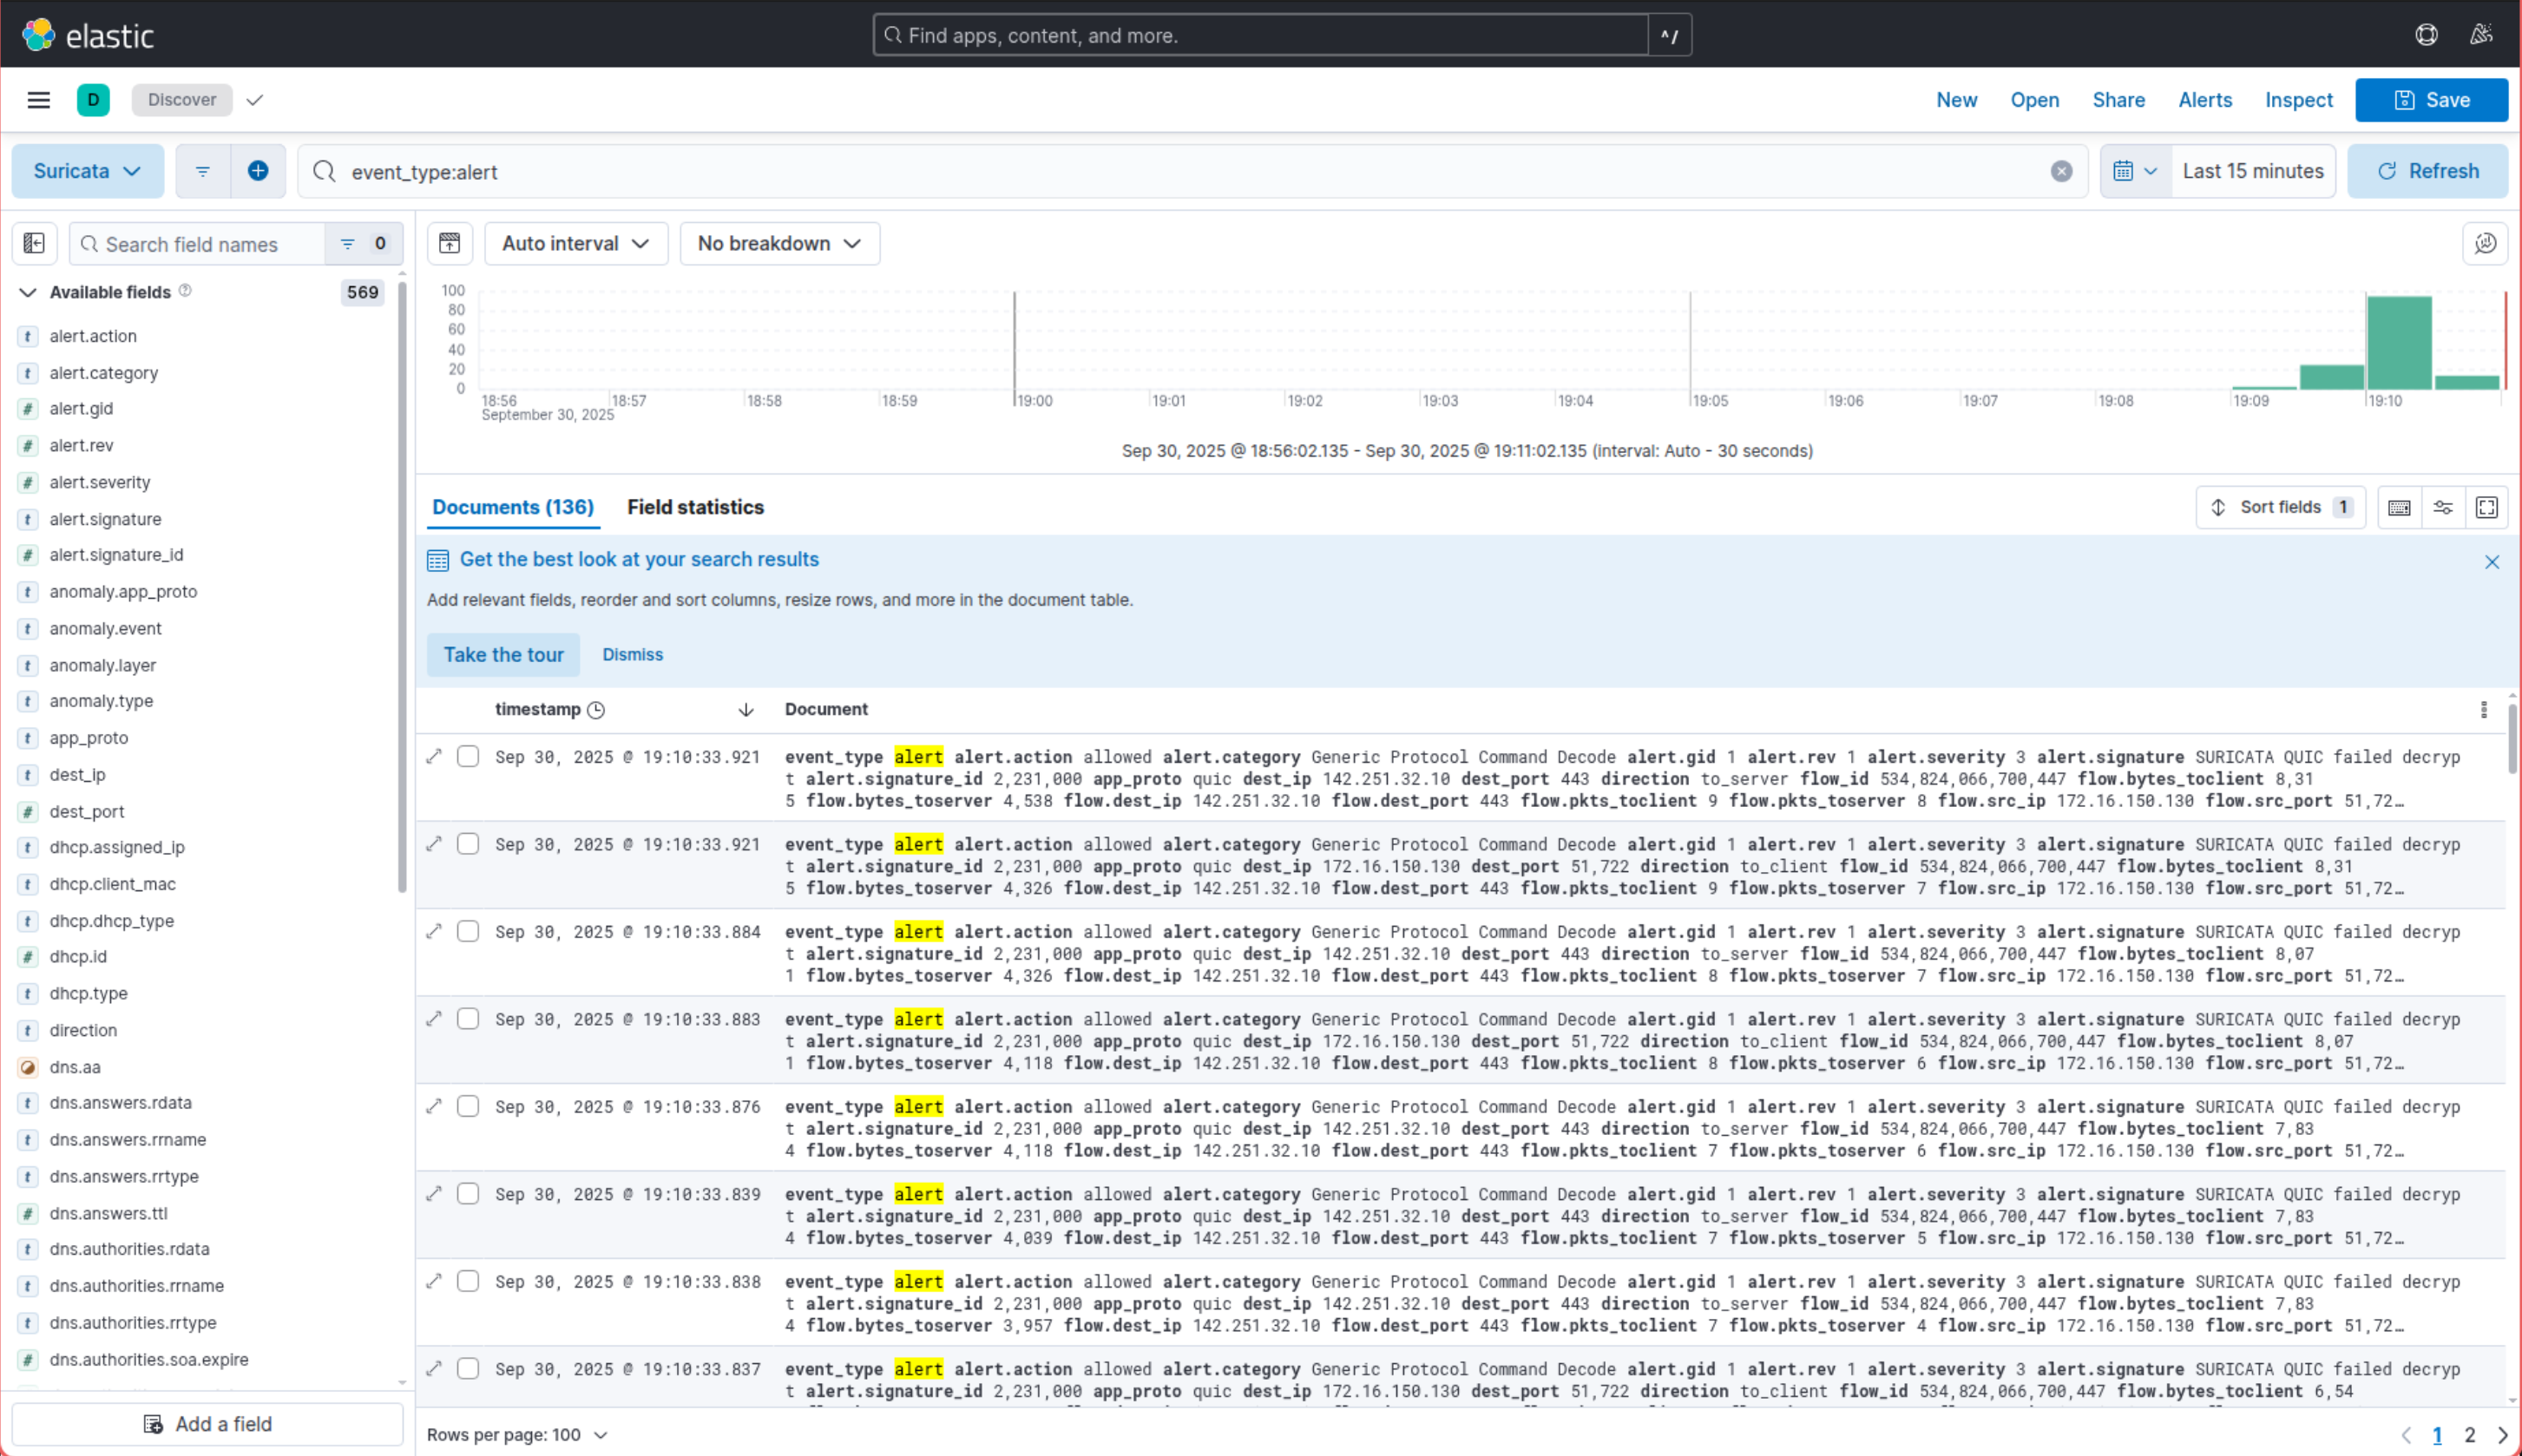
\includegraphics[width=0.70\linewidth]{assets/figures/kibana-discover.png}
    \caption{Affichage des événements Suricata dans Kibana Discover.}
\end{figure}

\bigskip
En résumé, \texttt{syslog-ng} assure avec succès son rôle de passerelle entre Suricata et Elasticsearch, en garantissant que chaque événement de sécurité est stocké localement puis rendu exploitable dans Kibana.

\section{Intégration des outils de visualisation}

Afin d’améliorer la visibilité et l’analyse des événements de sécurité, les journaux collectés par Suricata et envoyés via \texttt{syslog-ng} sont exploités dans Kibana. 
Cet outil permet de rechercher, filtrer et représenter graphiquement les alertes générées par l’IDS/IPS.

\subsection{Visualisation et tableaux de bord}
Kibana offre la possibilité de créer des graphiques et tableaux de bord personnalisés.  
Dans notre cas, nous avons réalisé une visualisation simple représentant le nombre d’alertes dans le temps.  
Ce test avait uniquement pour objectif de vérifier que toute la chaîne de collecte et d’intégration fonctionnait correctement (Suricata → syslog-ng → Elasticsearch → Kibana).
\begin{figure}[H]
    \centering
    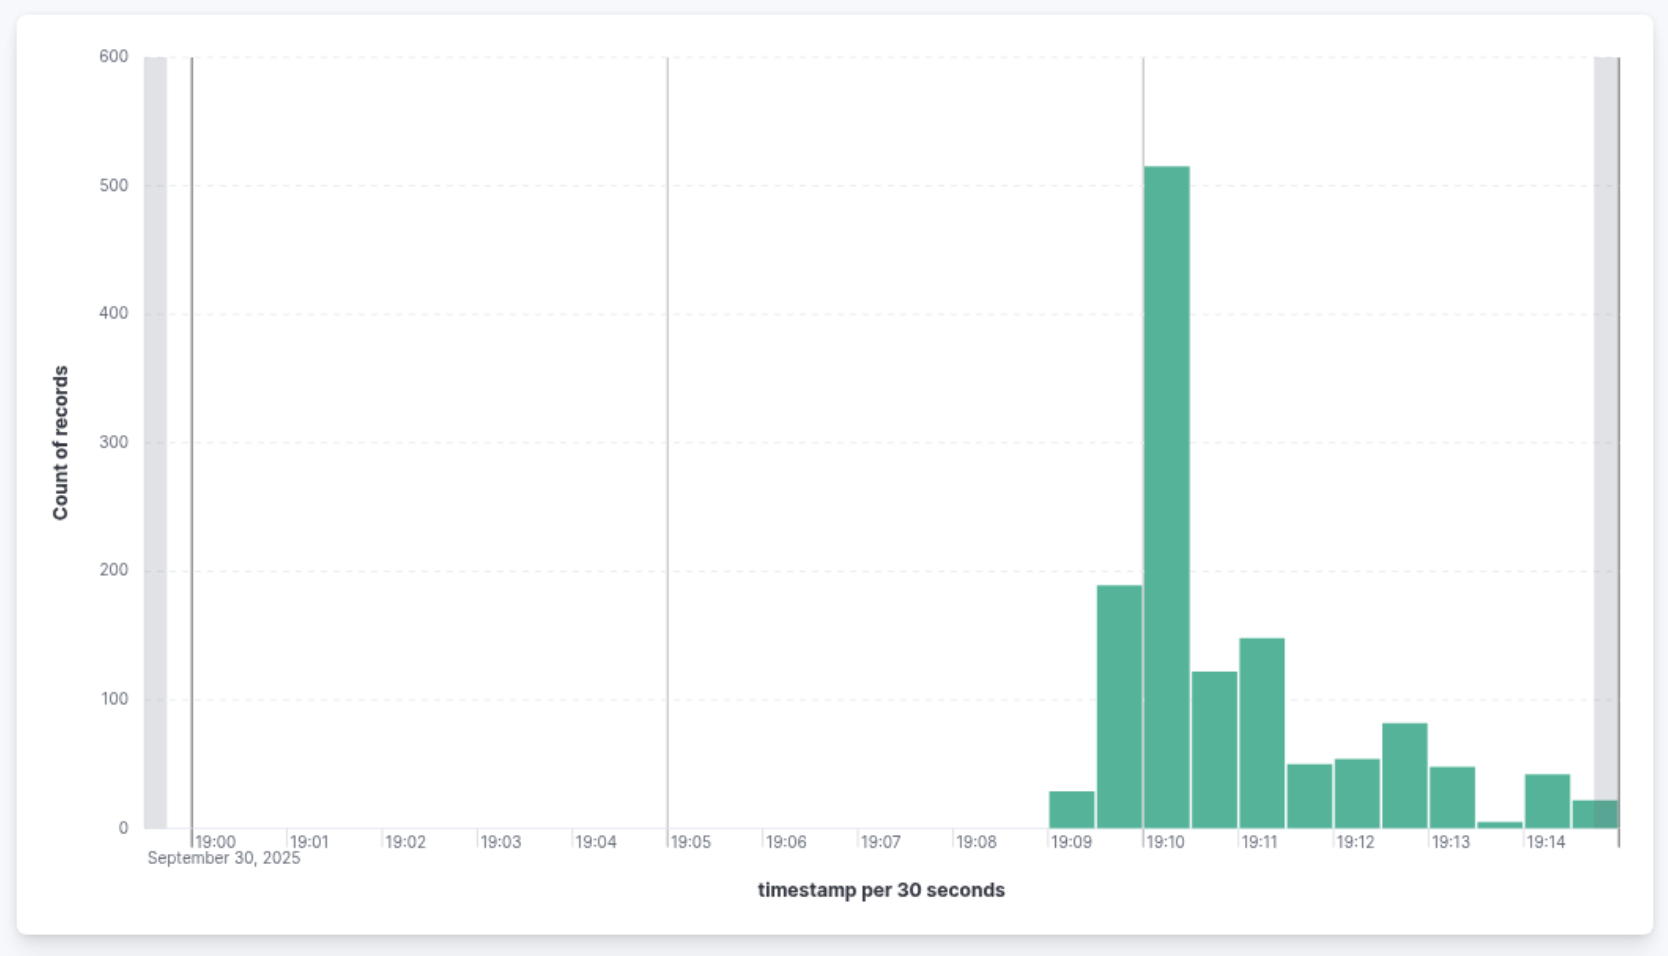
\includegraphics[width=0.65\linewidth]{assets/figures/kibana-dashboard.png}
    \caption{Exemple de visualisation des alertes Suricata dans Kibana.}
\end{figure}

\chapter{Scénarios d’intrusion (5 cas)}
\label{chap:chap_3}

\subsection{Scénario 1 — ICMP (ping)}
\textbf{Objectif :} Vérifier la capacité de l'IDS à détecter du trafic ICMP (ping).

\textbf{Justification :} Le ping est une méthode basique de reconnaissance utilisée pour confirmer la présence d'hôtes. Il s'agit d'un test simple permettant de valider la chaîne de détection (Suricata → syslog-ng → Elasticsearch → Kibana).

\textbf{Règle utilisée :}
\begin{lstlisting}[style=bashstyle]
alert icmp any any -> any any (msg:"ICMP test detected"; sid:1000001; rev:1;)
\end{lstlisting}

\textbf{Procédure :} exécution de \texttt{ping -c 6 8.8.8.8} depuis la VM.

\begin{figure}[H]
    \centering
    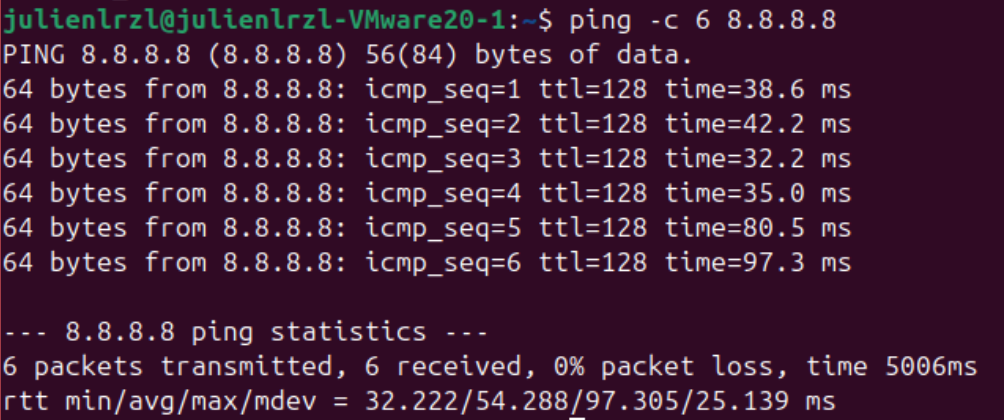
\includegraphics[width=0.9\linewidth]{assets/figures/scen1_ping_cmd.png}
    \caption{Commande \texttt{ping} exécutée dans le terminal (génération du trafic ICMP).}
    \label{fig:scen1_ping_cmd}
\end{figure}

\textbf{Preuves :} la figure \ref{fig:scen1_fastlog} montre l'entrée correspondante dans \path{/var/log/suricata/fast.log} et la figure \ref{fig:scen1_kibana} présente l'alerte remontée dans Kibana Discover.

\begin{figure}[H]
    \centering
    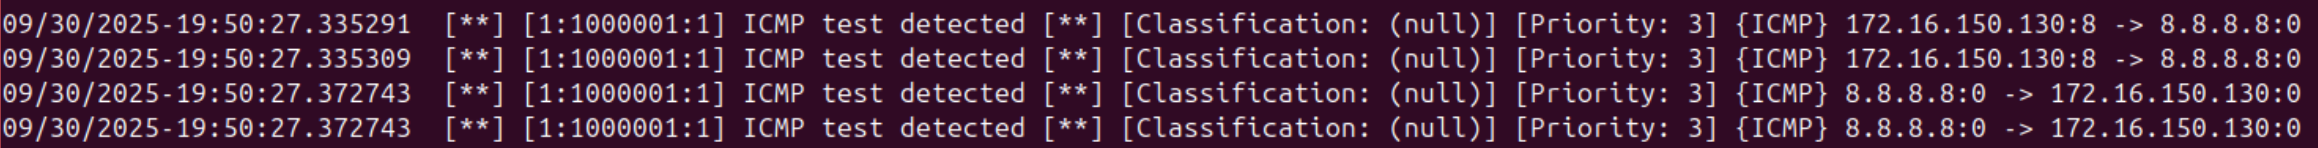
\includegraphics[width=0.9\linewidth]{assets/figures/scen1_fastlog.png}
    \caption{Alerte ICMP détectée par Suricata (extrait de fast.log).}
    \label{fig:scen1_fastlog}
\end{figure}

\begin{figure}[H]
    \centering
    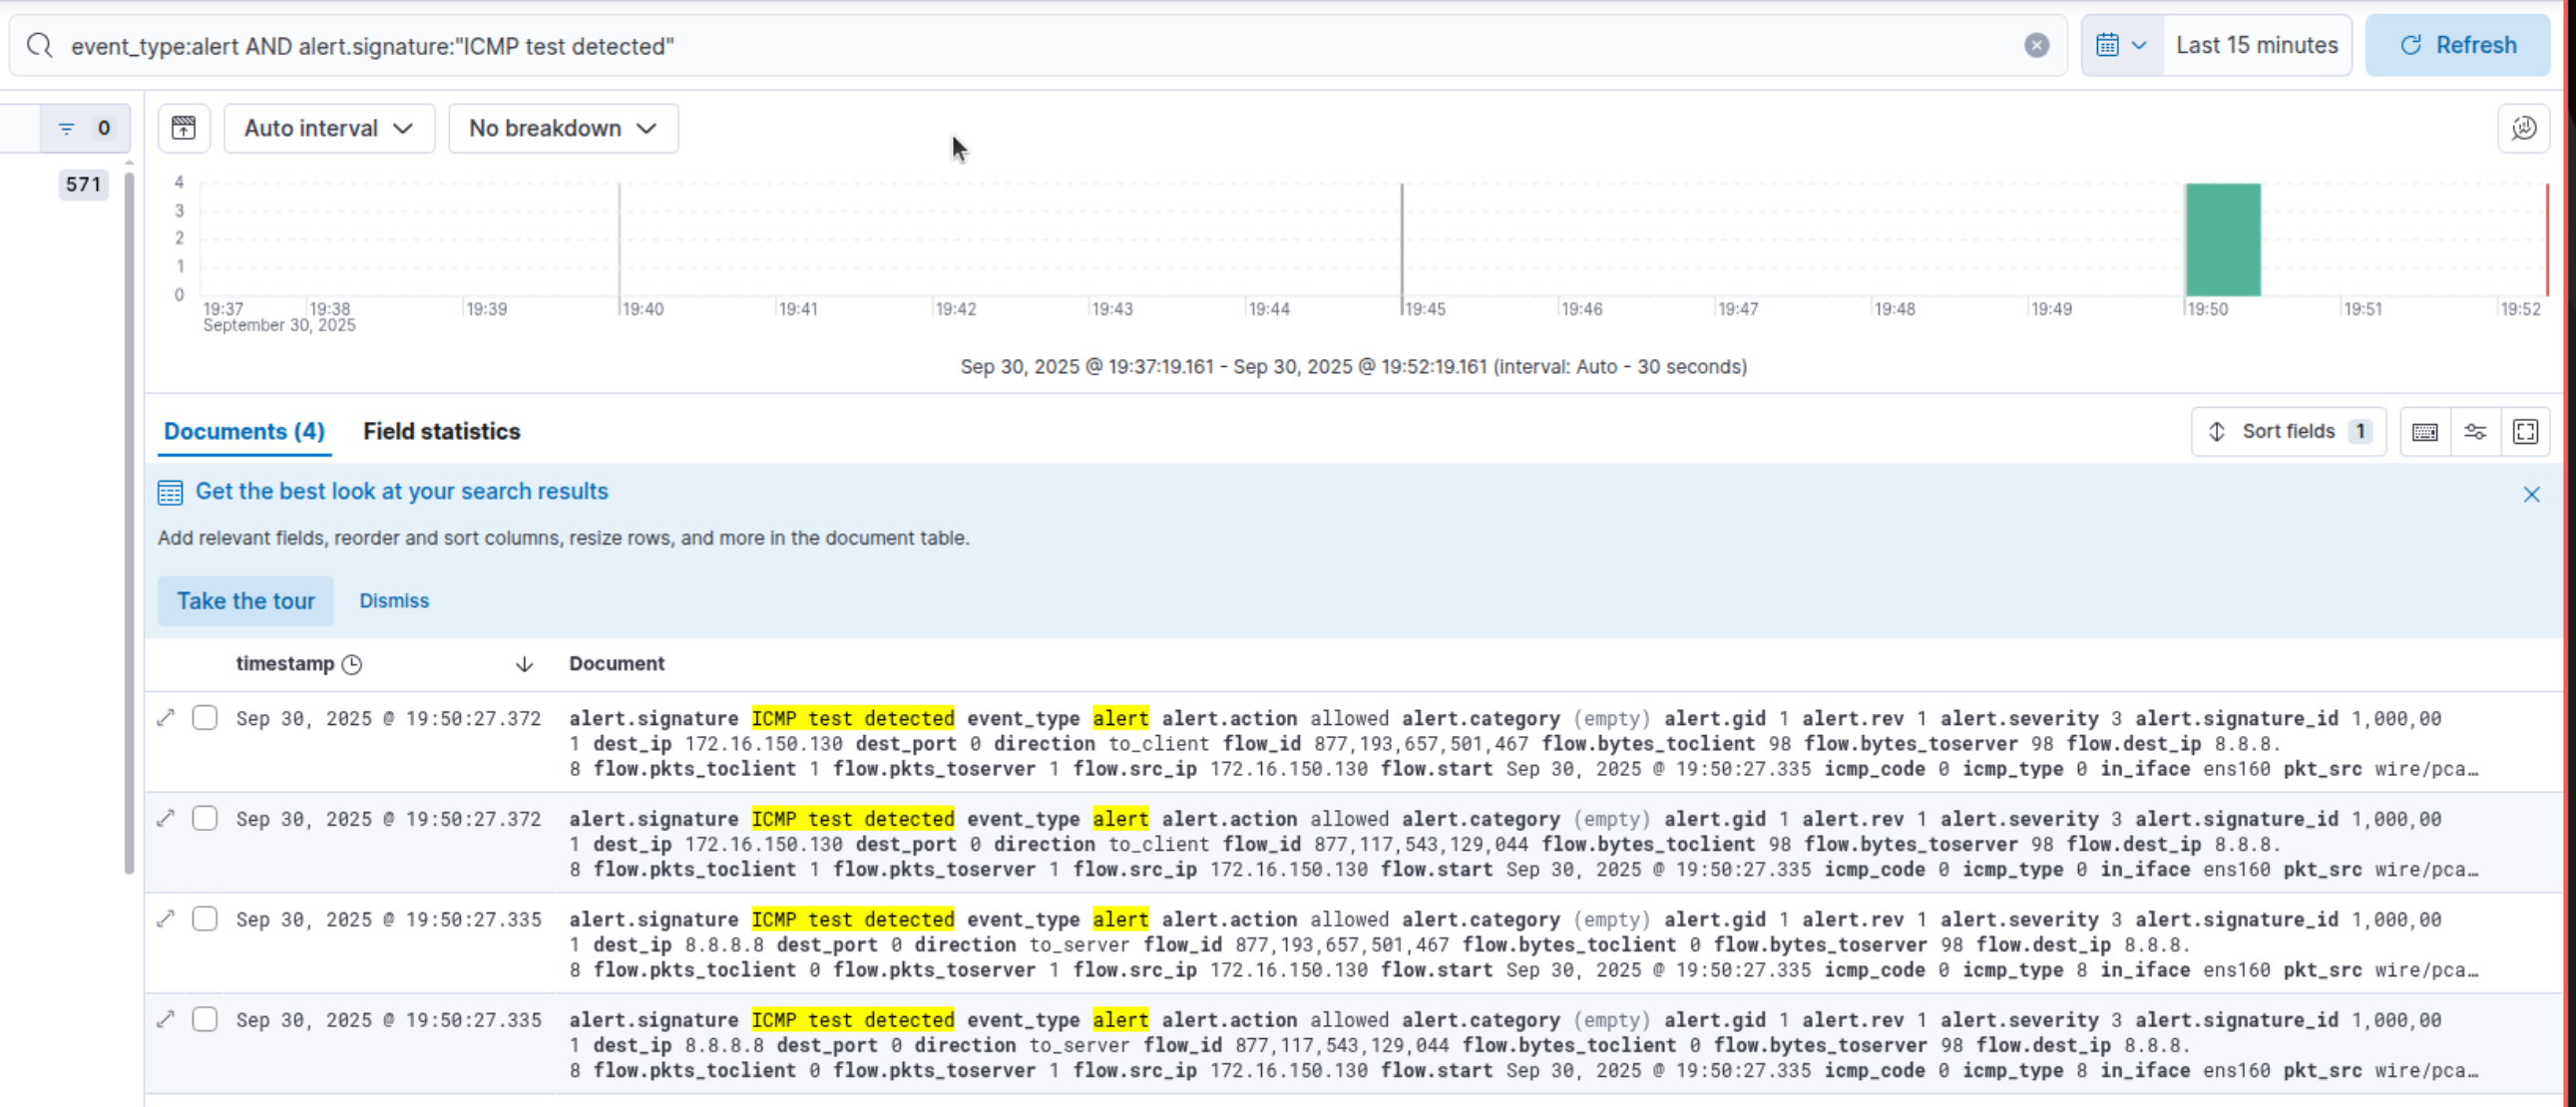
\includegraphics[width=0.9\linewidth]{assets/figures/scen1_kibana_discover.png}
    \caption{Alerte ICMP visible dans Kibana Discover.}
    \label{fig:scen1_kibana}
\end{figure}

\textbf{Utilité en conditions réelles :} le ping est utilisé par les administrateurs pour vérifier la disponibilité d’un hôte, mais aussi par des attaquants pour repérer des cibles actives lors de la phase de reconnaissance ; détecter et alerter sur ces requêtes permet de repérer des scans précoces et d'initier des mesures de durcissement ou de surveillance.

\clearpage
\subsection{Scénario 2 — Reconnaissance : scan Nmap}
\textbf{Objectif :} Détecter une activité de reconnaissance réseau (scan de ports).

\textbf{Justification :} Les scans de ports font partie des premières étapes d'une attaque : un attaquant cherche quels services sont exposés. Détecter ces scans permet d'anticiper des tentatives d'exploitation ultérieures.

\textbf{Règle utilisée :}
\begin{verbatim}
alert tcp any any -> any any (msg:"TCP portscan";
    threshold:type limit, track by_src, count 20, seconds 10;
    sid:1000004; rev:1;)
\end{verbatim}

\textbf{Procédure :} exécution d'un scan local depuis la VM :
\begin{verbatim}
sudo nmap -sS --top-ports 100 127.0.0.1
\end{verbatim}

\begin{figure}[H]
    \centering
    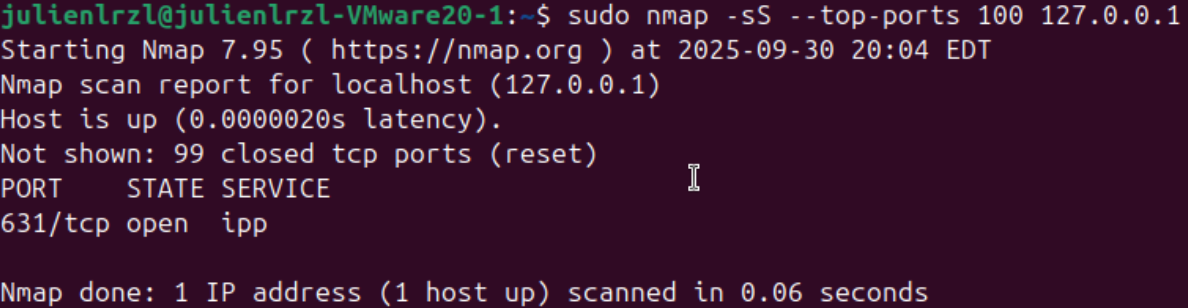
\includegraphics[width=0.9\linewidth]{assets/figures/scen2_nmap_cmd.png}
    \caption{Commande Nmap exécutée pour générer l'activité de reconnaissance.}
    \label{fig:scen2_nmap}
\end{figure}

\textbf{Preuves :} la figure \ref{fig:scen2_fastlog} montre l'entrée d'alerte correspondante dans \path{/var/log/suricata/fast.log} et la figure \ref{fig:scen2_kibana} présente les événements indexés et visibles dans Kibana Discover.

\begin{figure}[H]
    \centering
    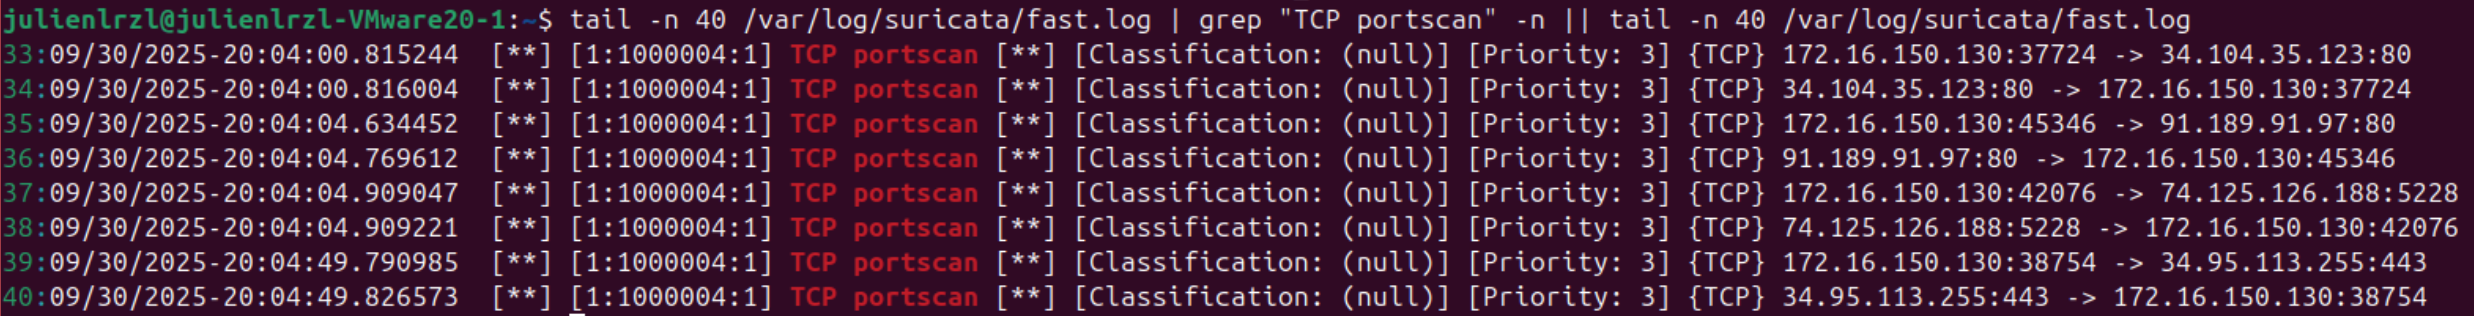
\includegraphics[width=0.9\linewidth]{assets/figures/scen2_fastlog.png}
    \caption{Alerte de type \texttt{TCP portscan} détectée par Suricata (extrait de fast.log).}
    \label{fig:scen2_fastlog}
\end{figure}

\begin{figure}[H]
    \centering
    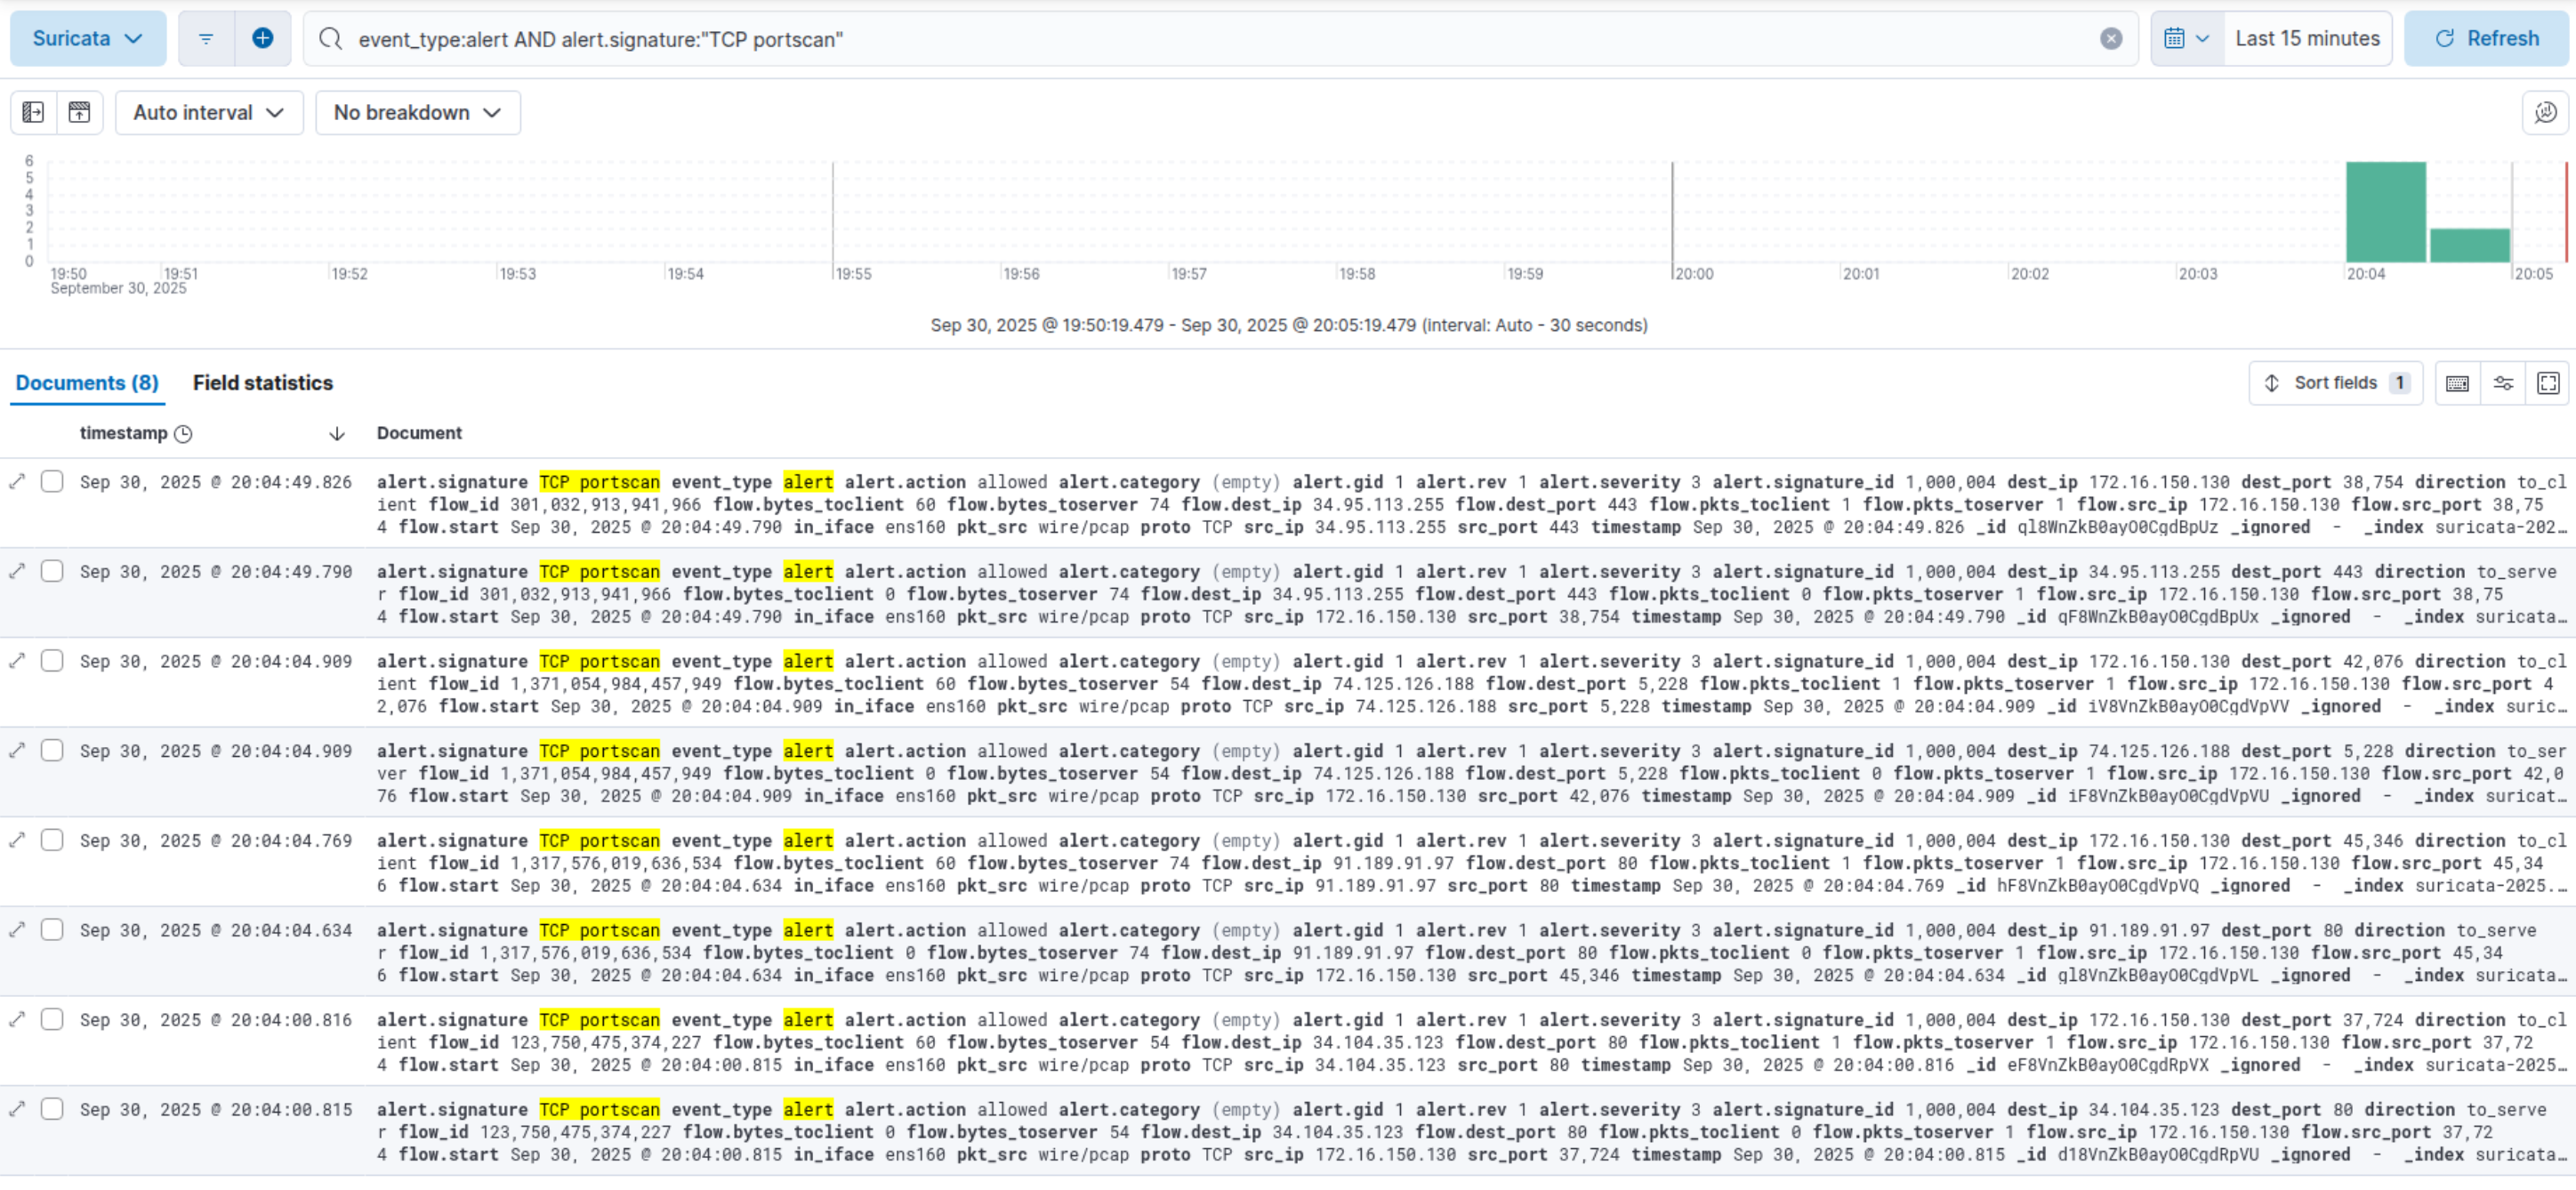
\includegraphics[width=0.9\linewidth]{assets/figures/scen2_kibana_discover.png}
    \caption{Evénements \texttt{TCP portscan} visibles dans Kibana Discover.}
    \label{fig:scen2_kibana}
\end{figure}

\textbf{Analyse :} L'alerte confirme la détection d'une activité de reconnaissance. En environnement réel, la détection précoce d'un scan permet de déclencher des contre-mesures (blocage d'IP, investigation, enrichissement des logs).

\clearpage
\subsection{Scénario 3 — Tentatives SSH}
\textbf{Objectif :} Détecter des connexions SSH (et potentiellement des tentatives de brute-force).

\textbf{Justification :} Le protocole SSH est chiffré et ne peut pas être analysé en profondeur par l’IDS. Néanmoins, il est possible de détecter les tentatives de connexion sur le port 22, ainsi que des patterns anormaux de connexions répétées, ce qui peut indiquer une attaque par force brute.

\textbf{Règles utilisées :}
\begin{lstlisting}[style=bashstyle]
alert tcp $EXTERNAL_NET any -> $HOME_NET 22 (msg:"Possible SSH brute forcing!"; flags: S+; threshold: type both, track by_src, count 5, seconds 30; sid:10000001; rev: 1;)
\end{lstlisting}

\textbf{Procédure :} génération de connexions TCP vers le port 22 en boucle, simulant des tentatives répétées de connexion SSH :
\begin{verbatim}
for i in $(seq 1 10); do nc -vz 172.16.150.130 22; sleep 0.3; done
\end{verbatim}

\begin{figure}[H]
    \centering
    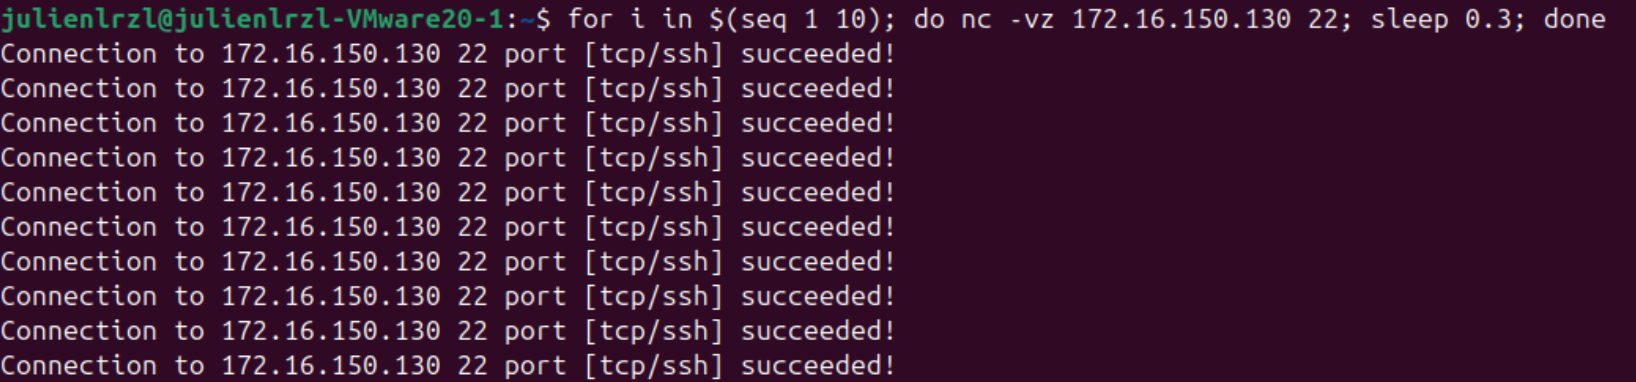
\includegraphics[width=0.9\linewidth]{assets/figures/scen3_nc_cmd.png}
    \caption{Commande \texttt{nc} utilisée pour simuler des connexions SSH répétées sur le port 22.}
    \label{fig:scen3_nc_cmd}
\end{figure}

\textbf{Preuves :} la figure \ref{fig:scen3_fastlog} montre l’entrée d’alerte dans \path{/var/log/suricata/fast.log} et la figure \ref{fig:scen3_kibana} présente l’événement visible dans Kibana Discover.

\begin{figure}[H]
    \centering
    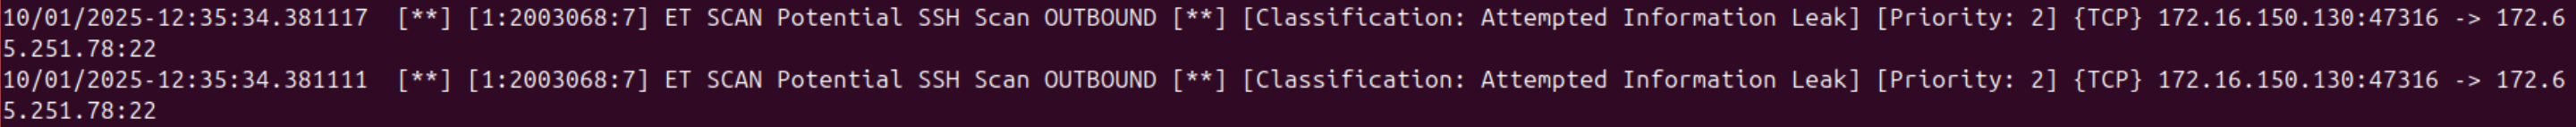
\includegraphics[width=0.9\linewidth]{assets/figures/scen3_fastlog.png}
    \caption{Alertes SSH détectées par Suricata (extrait de fast.log).}
    \label{fig:scen3_fastlog}
\end{figure}

\begin{figure}[H]
    \centering
    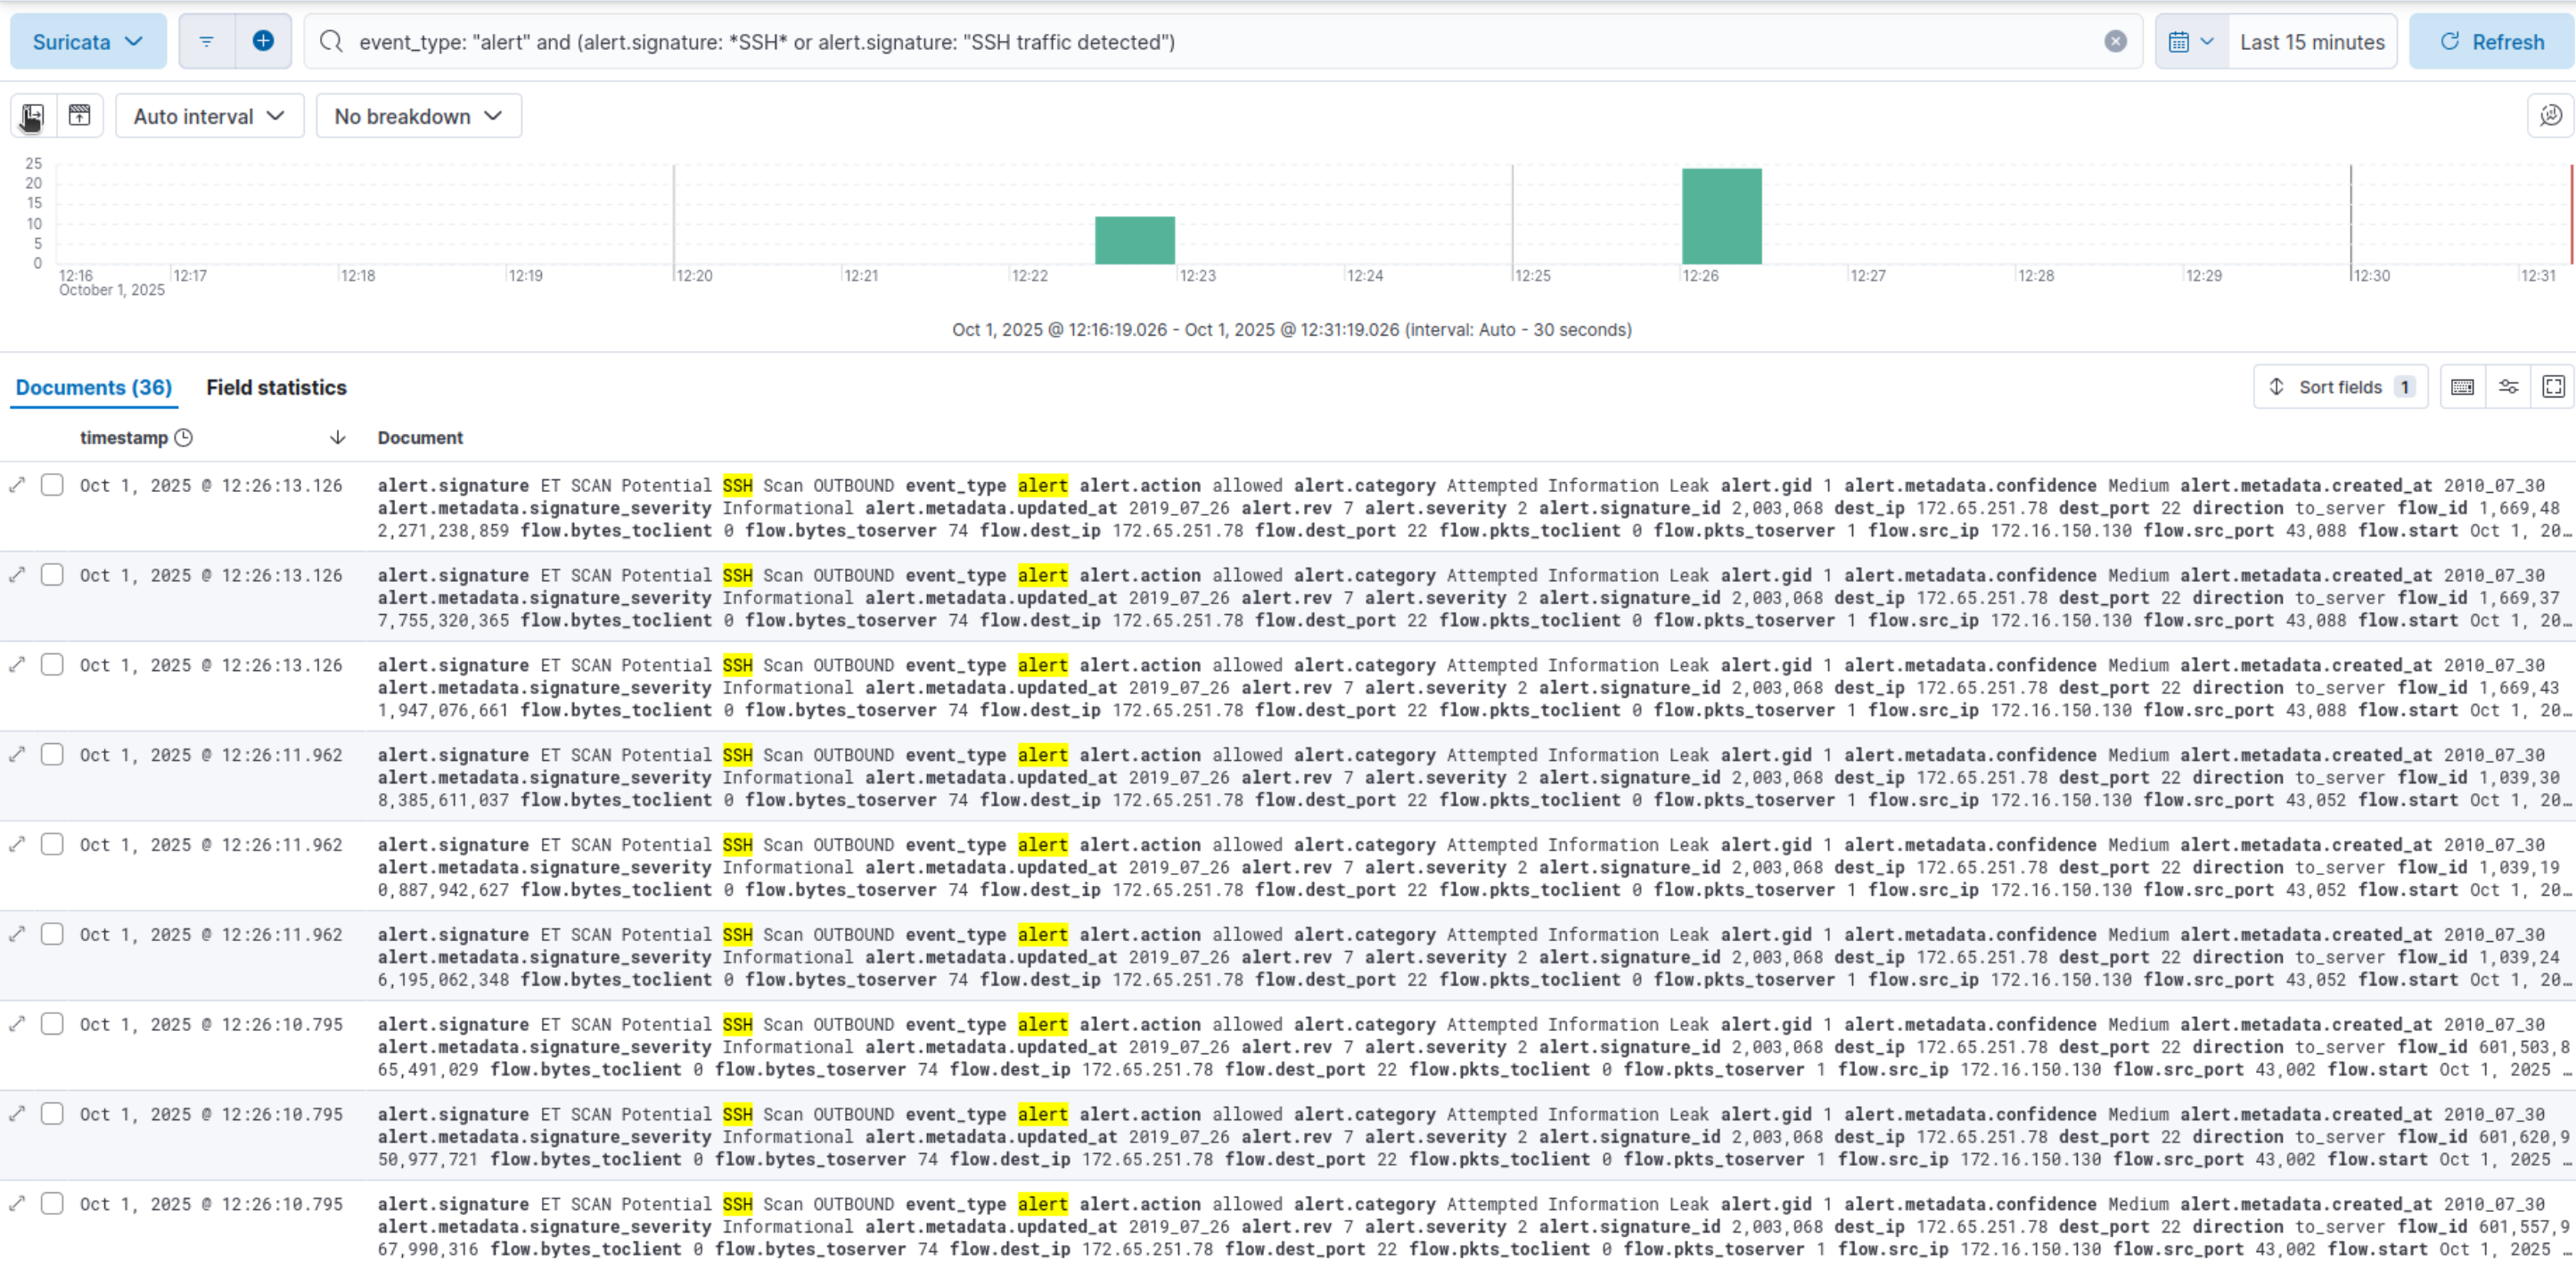
\includegraphics[width=0.9\linewidth]{assets/figures/scen3_kibana.png}
    \caption{Événements SSH détectés dans Kibana Discover.}
    \label{fig:scen3_kibana}
\end{figure}

\textbf{Analyse :}  
Les alertes confirment que Suricata détecte bien le trafic SSH sur le port 22.  
Dans un contexte réel, cela permet de repérer rapidement des tentatives suspectes (par exemple un outil d’attaque par dictionnaire). Même si le contenu SSH reste chiffré, la corrélation entre fréquence et volume des connexions permet d’identifier un comportement anormal. Couplé aux logs système d’authentification (\path{/var/log/auth.log}), cela permet de confirmer une tentative de brute-force.

\clearpage
\subsection{Scénario 4 — Fuzzing web (volume élevé)}
\textbf{Objectif :} Détecter un volume anormalement élevé de requêtes HTTP provenant d'une même source (possible fuzzing / scanner web).

\textbf{Règle utilisée :}
\begin{lstlisting}[style=bashstyle]
alert http any any -> any any (
  msg:"WEB-FUZZ - High HTTP request rate from source (possible fuzzing)";
  flow:to_server,established;
  detection_filter: track by_src, count 100, seconds 60;
  sid:1002001; rev:1; classtype:attempted-recon; priority:2;
)
\end{lstlisting}

\textbf{Procédure :}
\begin{lstlisting}[style=bashstyle]
seq 1 200 | xargs -n1 -P20 -I{} curl -s -o /dev/null "http://172.16.150.130:5601/index.html"
\end{lstlisting}

\textbf{Preuves :} la figure \ref{fig:scen4_fastlog} montre l’alerte dans \path{/var/log/suricata/fast.log} et la figure \ref{fig:scen4_kibana_discover} l’événement indexé et visible dans Kibana Discover.

\begin{figure}[H]
    \centering
    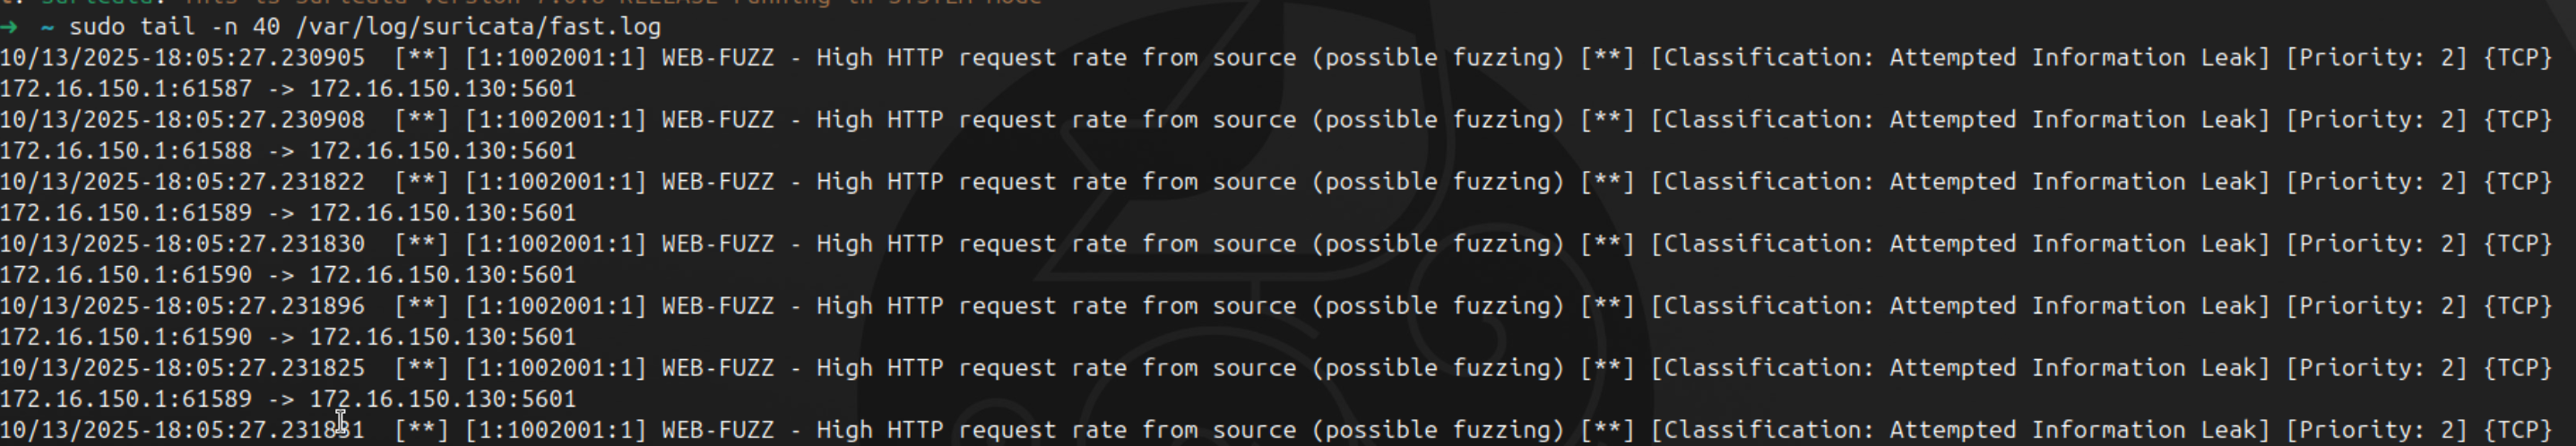
\includegraphics[width=0.9\linewidth]{assets/figures/scen4_fastlog.png}
    \caption{Alerte \texttt{WEB-FUZZ} détectée par Suricata (extrait de fast.log).}
    \label{fig:scen4_fastlog}
\end{figure}

\begin{figure}[H]
    \centering
    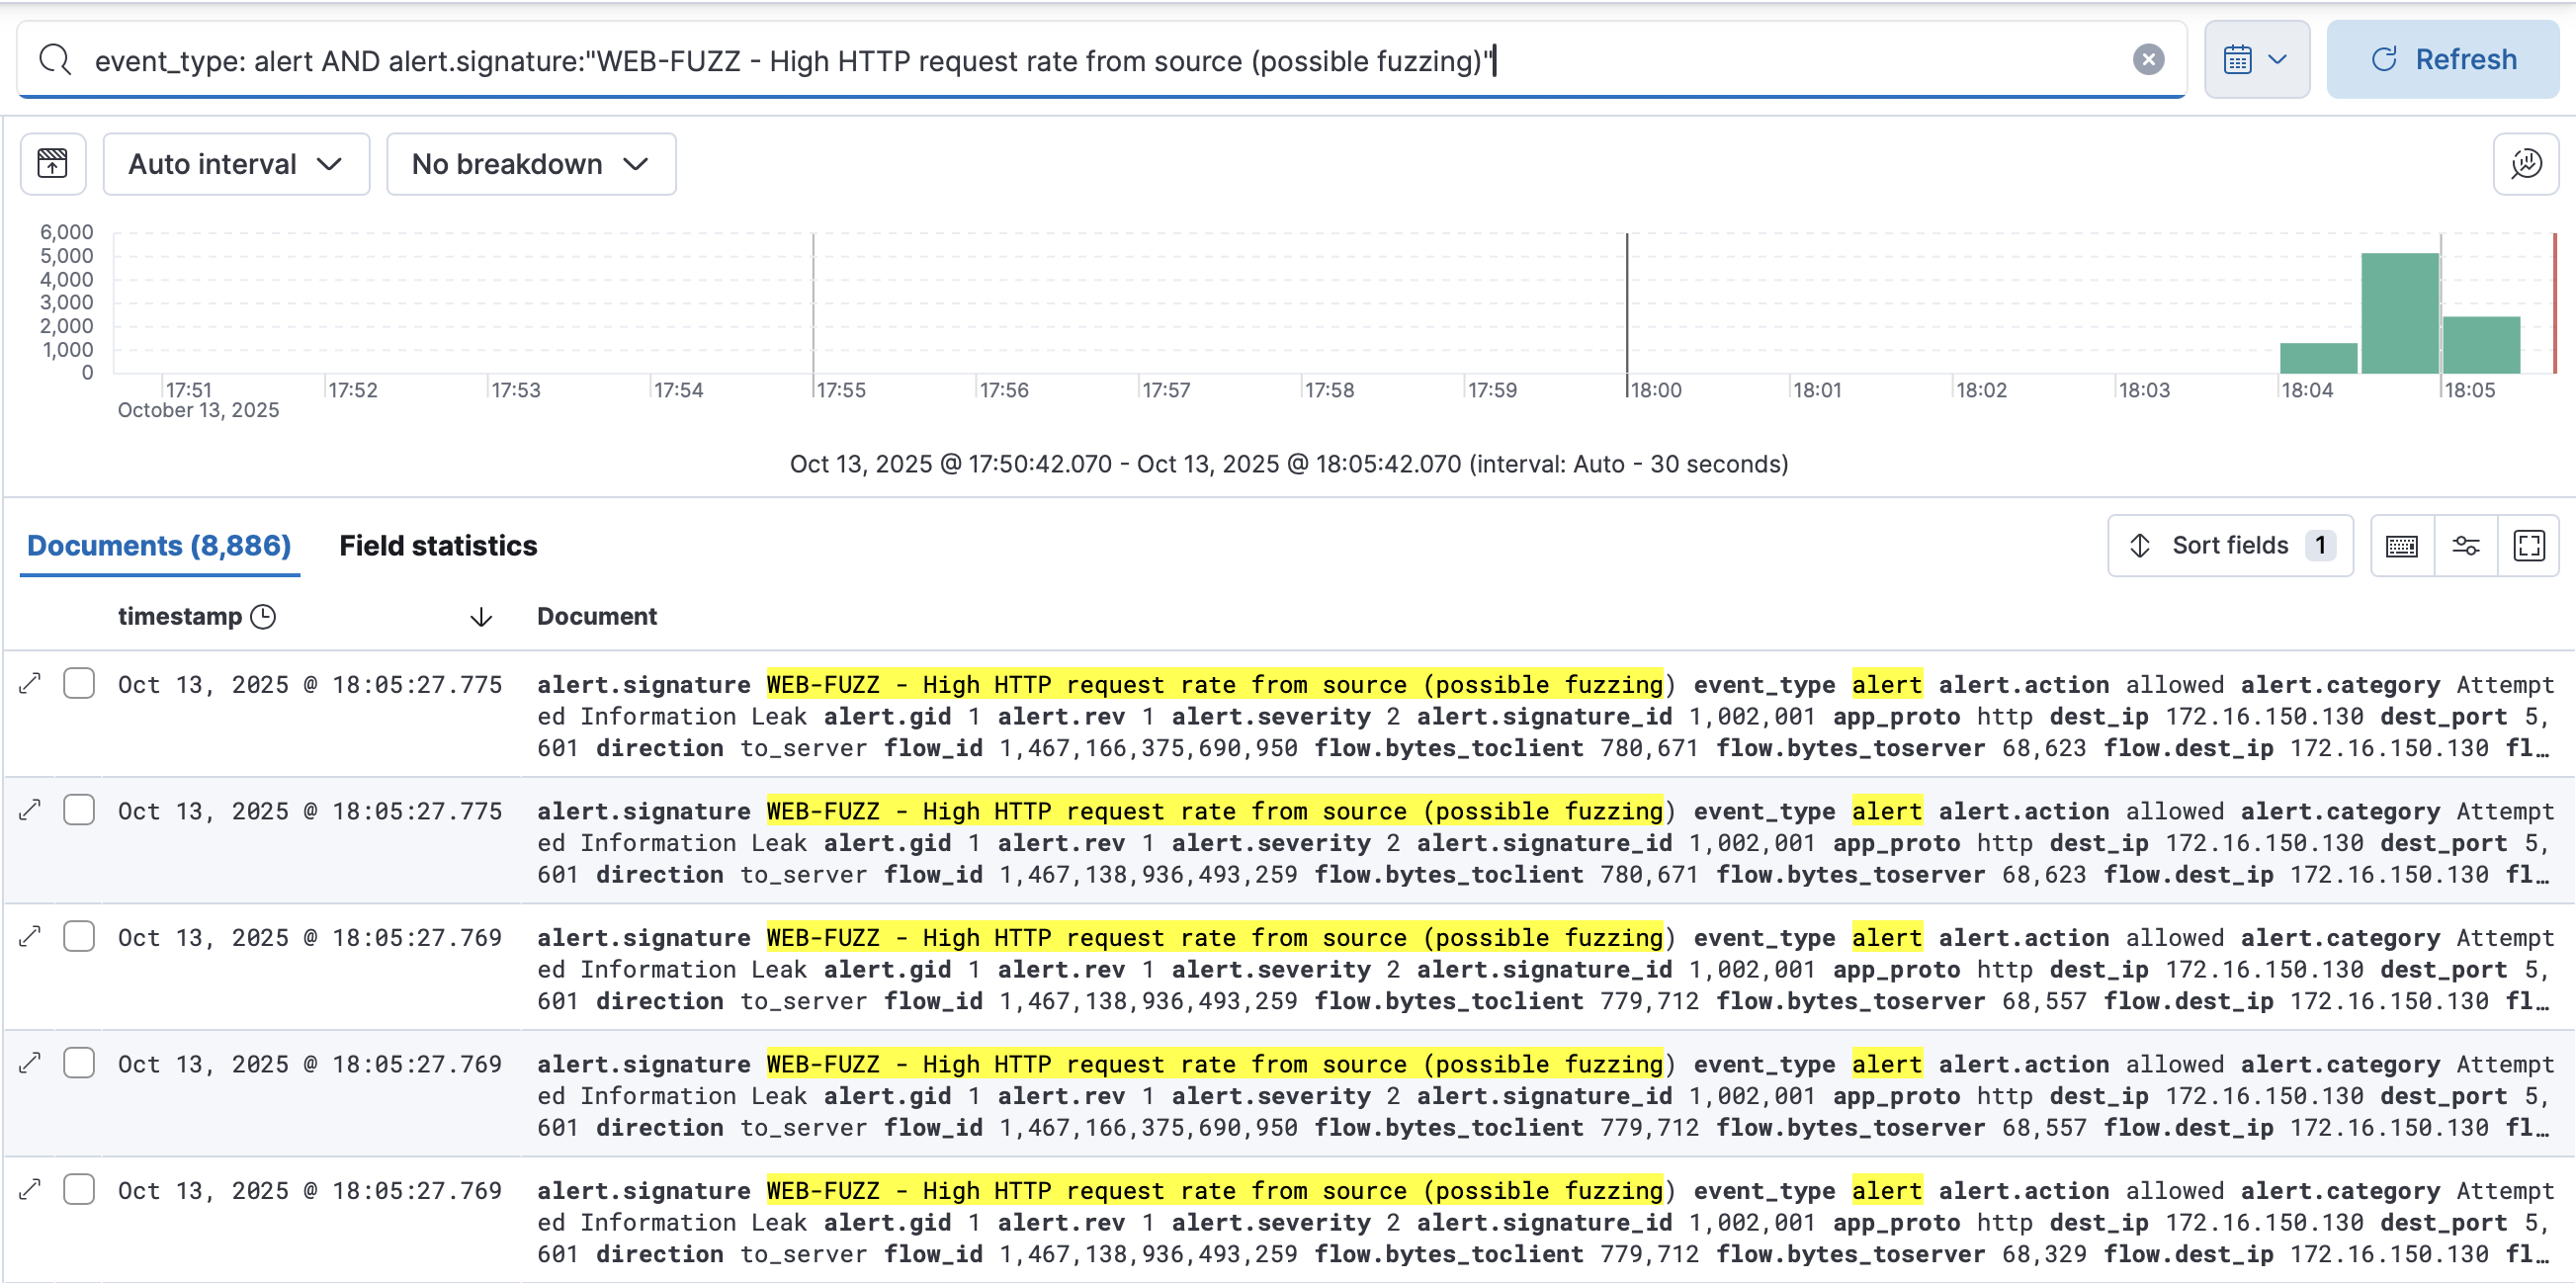
\includegraphics[width=0.9\linewidth]{assets/figures/scen4_kibana_discover.png}
    \caption{Evénement \texttt{WEB-FUZZ} indexé et visible dans Kibana Discover.}
    \label{fig:scen4_kibana_discover}
\end{figure}

\textbf{Analyse :} Cette règle est utile pour repérer des scans/fuzzing orientés web. En production, attention aux faux positifs (par ex. tests de charge légitimes) : corréler à des sources connues et ajuster seuils. Combiner cette règle avec des logs d’accès web et des systèmes de blocage automatique (Fail2Ban / WAF) améliore la réponse.

\clearpage
\subsection{Scénario 5 — FTP : tentative d'accès anonyme}
\textbf{Objectif :} Détecter une tentative d'accès FTP en mode anonyme (login \texttt{anonymous}), typique d’un accès public ou d’un test de découverte de services.

\textbf{Justification :} Les serveurs FTP mal configurés autorisant l'accès anonyme peuvent être utilisés pour exfiltrer ou déposer des fichiers. Détecter les tentatives \texttt{USER anonymous} permet d'identifier des services exposés ou des tests automatisés d'accès.

\textbf{Règle utilisée :}
\begin{lstlisting}[style=bashstyle]
alert tcp any any -> any 21 (msg:"FTP anonymous login attempt"; \
content:"USER anonymous"; nocase; sid:1003001; rev:1;)
\end{lstlisting}

\textbf{Procédure :} exécution de la commande FTP en mode anonyme depuis l'exterieur :
\begin{lstlisting}[style=bashstyle]
    nc -vz 172.16.150.130 21
\end{lstlisting}

\textbf{Preuves :} la figure \ref{fig:scen_ftp_fastlog} montre l’alerte dans \path{/var/log/suricata/fast.log} et la figure \ref{fig:scen_ftp_kibana} l’événement remonté dans Kibana Discover.

\begin{figure}[H]
    \centering
    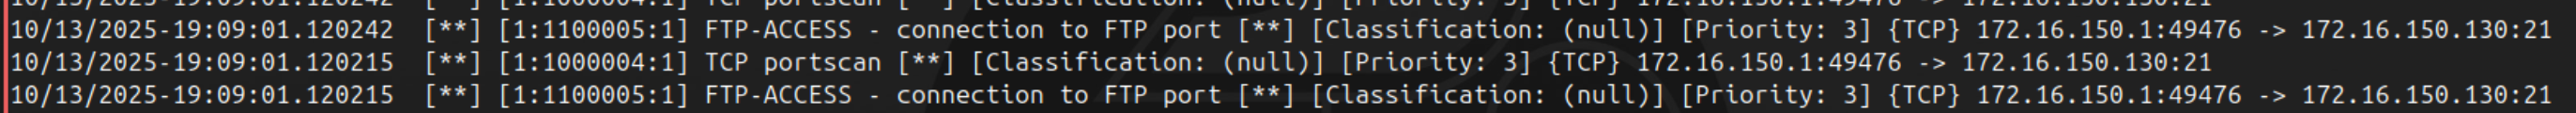
\includegraphics[width=0.9\linewidth]{assets/figures/scen_ftp_fastlog.png}
    \caption{Alerte \texttt{FTP anonymous login attempt} détectée par Suricata (extrait de fast.log).}
    \label{fig:scen_ftp_fastlog}
\end{figure}

\begin{figure}[H]
    \centering
    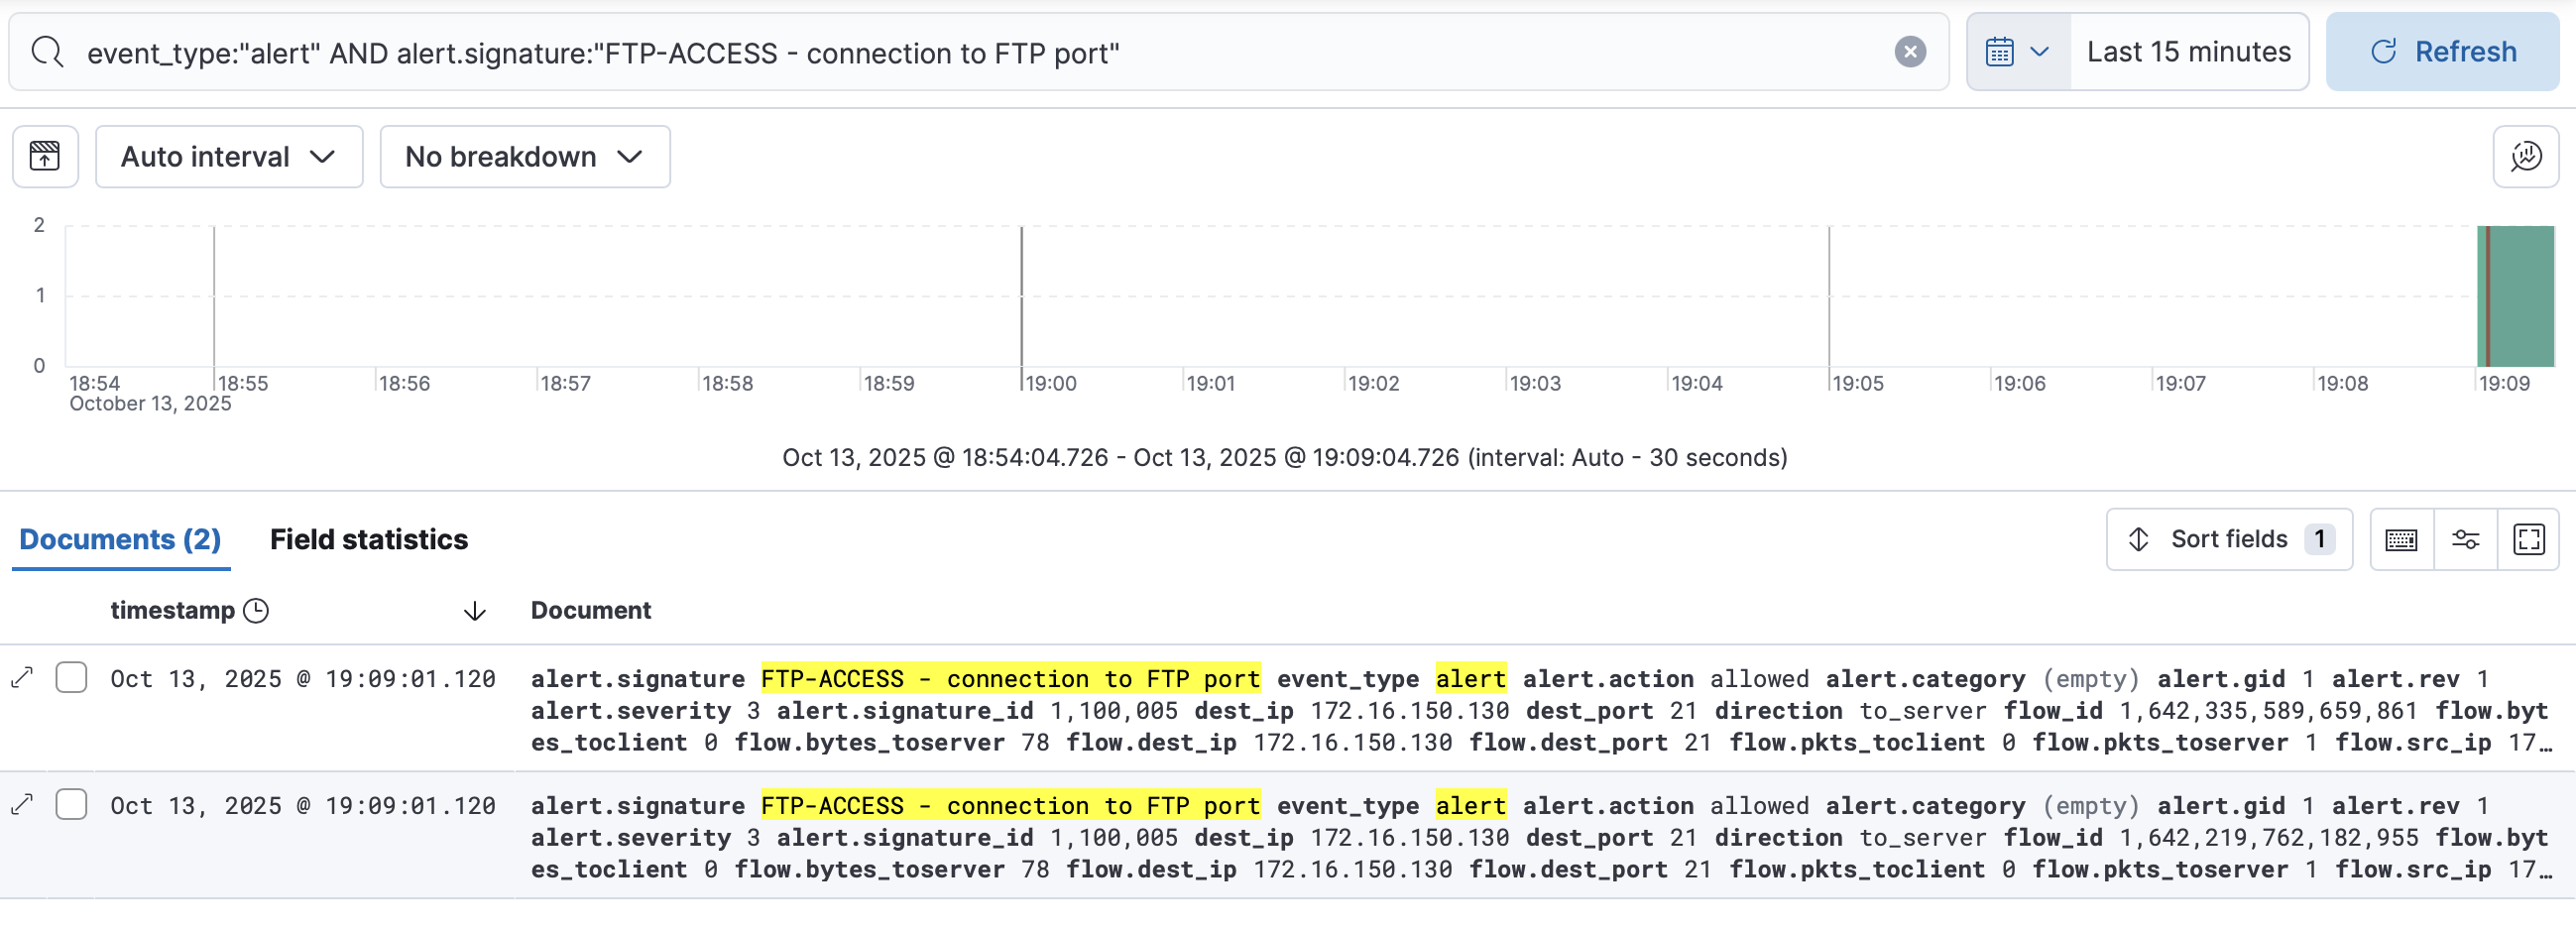
\includegraphics[width=0.9\linewidth]{assets/figures/scen_ftp_kibana.png}
    \caption{Evénement FTP anonyme visible dans Kibana Discover.}
    \label{fig:scen_ftp_kibana}
\end{figure}

\textbf{Analyse :}  
La règle détecte l’envoi explicite du login \texttt{USER anonymous}. En production, il faudra :
\begin{itemize}
  \item réduire les faux positifs en corrélant avec les logs du service FTP (\path{/var/log/vsftpd.log} ou \path{/var/log/auth.log}) ;
  \item éventuellement améliorer la règle (par exemple détection de \texttt{PASS} faibles, détection de transferts après login anonyme, ou surveillance d'un grand nombre de fichiers transférés) ;
  \item si nécessaire, bloquer automatiquement l’IP source (via firewall / fail2ban) ou désactiver l’anonymous sur le serveur.
\end{itemize}
\chapter{Visualisation et alertes}
\label{chap:chap_4}

\section{Collecte et gestion des logs prioritaires en sécurité}

Comme détaillé dans le chapitre précédent, le système de détection d’intrusion (Suricata) génère en continu des journaux relatifs aux activités réseau.  
Ces logs sont collectés et centralisés via syslog-ng, puis transmis à Elasticsearch pour être analysés et visualisés dans Kibana.  
Cette chaîne (Suricata → syslog-ng → Elasticsearch → Kibana) assure la traçabilité complète des événements de sécurité observés lors des cinq scénarios d’intrusion précédemment simulés.

\subsection{Collecte et transfert des journaux}

Les journaux produits par Suricata sont stockés dans le répertoire \path{/var/log/suricata/}.  
On distingue principalement deux fichiers :
\begin{itemize}
  \item \texttt{fast.log} : enregistre les alertes textuelles (lisibles directement dans le terminal) ;
  \item \texttt{eve.json} : contient l’ensemble des événements au format JSON, destiné à être lu par \texttt{syslog-ng} pour transfert vers la base \texttt{Elasticsearch}.
\end{itemize}

Afin de vérifier que le processus de collecte est bien actif, la commande suivante permet d’observer que \texttt{syslog-ng} lit en continu le fichier \texttt{eve.json} :
\begin{verbatim}
sudo lsof /var/log/suricata/eve.json
\end{verbatim}

\begin{figure}[H]
    \centering
    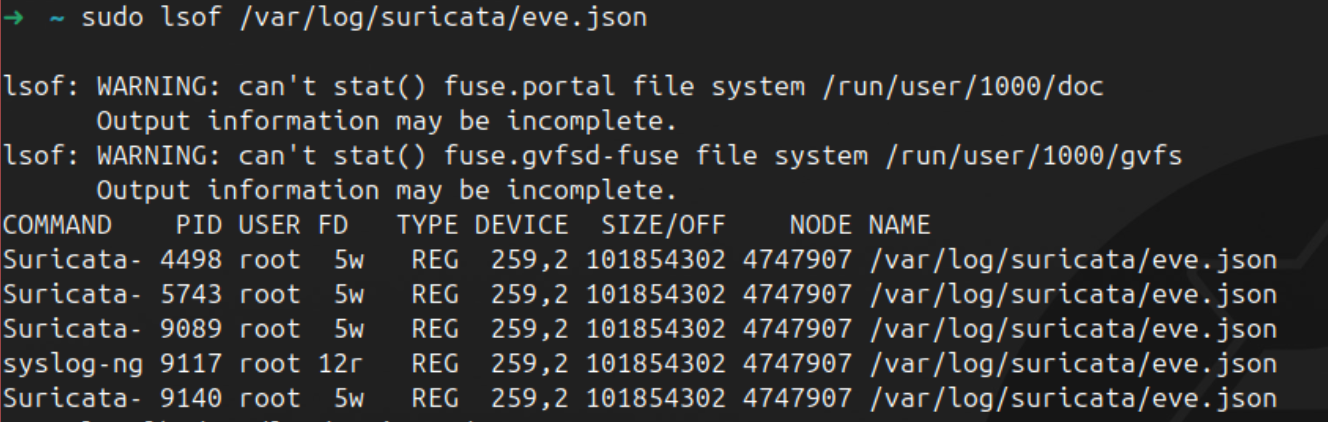
\includegraphics[width=0.9\linewidth]{assets/figures/syslog_ng_evejson.png}
    \caption{Vérification du flux de collecte : \texttt{syslog-ng} lit en continu \texttt{eve.json}.}
    \label{fig:syslog_ng_evejson}
\end{figure}

\subsection{Structure et rotation automatique des logs}

Les fichiers de journaux sont automatiquement gérés par le service logrotate, qui effectue périodiquement une rotation et une compression des anciens fichiers.  
Cela garantit une conservation historique tout en évitant la saturation du disque.

La commande suivante permet de visualiser cette rotation automatique :
\begin{verbatim}
ls -lh /var/log/suricata/
\end{verbatim}

\begin{figure}[H]
    \centering
    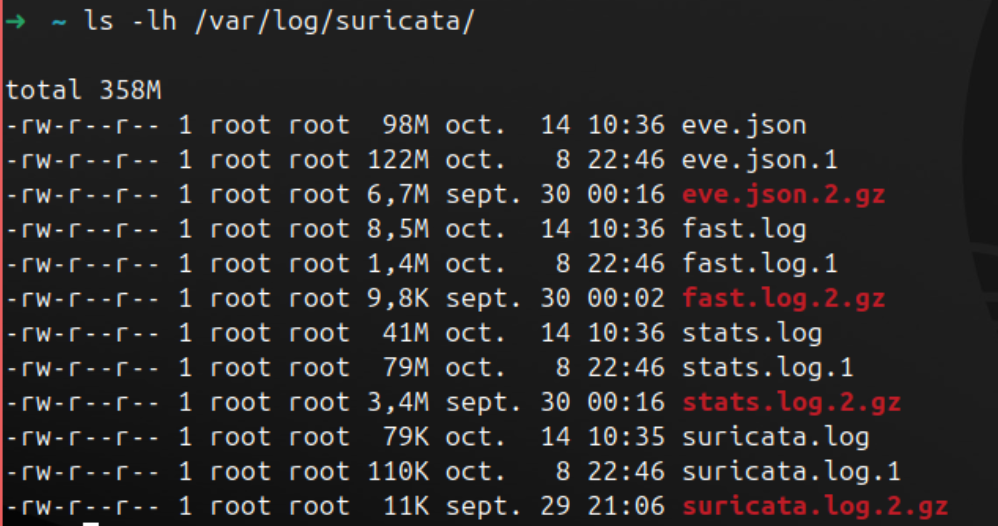
\includegraphics[width=0.75\linewidth]{assets/figures/suricata_logs_rotation.png}
    \caption{Rotation automatique et compression des journaux dans \texttt{/var/log/suricata/}.}
    \label{fig:suricata_logs_rotation}
\end{figure}

Les fichiers actifs portent l’extension \texttt{.log}, tandis que les précédents sont numérotés (\texttt{.log.1}) et les plus anciens compressés (\texttt{.log.2.gz}).  
Cette rotation automatique est essentielle pour maintenir la disponibilité et la fiabilité des logs dans le temps.

\subsection{Corrélation et visualisation dans Kibana}

Les événements issus de Suricata sont ensuite indexés dans Elasticsearch et visualisés dans Kibana Discover.  
Chaque alerte correspond à une signature spécifique (champ \texttt{alert.signature}) générée par l’une des règles locales définies pour les scénarios ICMP, Nmap, SSH, Web Fuzzing et FTP comme on l'a vu dans les chapitres précédents du rapport.

\subsection{Synthèse de la collecte par scénario}

\begin{table}[H]
\centering
\begin{tabular}{|l|l|l|}
\hline
\textbf{Scénario d’intrusion} & \textbf{Type d’événement détecté} & \textbf{Fichiers de logs concernés} \\ \hline
1 — ICMP (Ping) & Trafic ICMP (echo request/reply) & fast.log / eve.json \\ \hline
2 — Scan Nmap & Connexions TCP multiples & fast.log / eve.json \\ \hline
3 — SSH & Connexions répétées sur le port 22 & fast.log / eve.json \\ \hline
4 — Web Fuzzing & Volume élevé de requêtes HTTP & fast.log / eve.json \\ \hline
5 — FTP Anonyme & Connexion au port 21 (anonymous login) & fast.log / eve.json \\ \hline
\end{tabular}
\caption{Correspondance entre les scénarios d’intrusion et les types de logs collectés.}
\label{tab:scen_logs}
\end{table}

\subsection{Justification et intérêt sécurité}

Ce mécanisme de collecte et de gestion centralisée offre plusieurs avantages essentiels :
\begin{itemize}
    \item \textbf{Détection précoce des comportements anormaux}, grâce à la corrélation des alertes entre différents protocoles ;
    \item \textbf{Préservation des preuves techniques} (traçabilité et audit post-incident) ;
    \item \textbf{Hiérarchisation des menaces} via la priorité et le niveau de sévérité des logs ;
    \item \textbf{Surveillance continue et automatique}, assurée par la rotation et la centralisation.
\end{itemize}

\clearpage
\section{Point bonus — Tableau de bord Kibana personnalisé}

\textbf{Objectif :} Créer un tableau de bord Kibana personnalisé afin de visualiser en temps réel les alertes issues de Suricata et de synthétiser les cinq scénarios d'intrusion précédemment mis en œuvre.

\textbf{Procédure de création :}
\begin{enumerate}
    \item Dans Kibana, accéder à \textbf{Analytics → Dashboard → Create new dashboard}.
    \item Ajouter les visualisations sauvegardées depuis la bibliothèque (\texttt{Add from library}), notamment :
    \begin{itemize}
        \item \textbf{KPI – Total alerts} : affiche le nombre total d’alertes détectées ;
        \item \textbf{Alerts over time} : courbe temporelle représentant l’évolution des alertes ;
        \item \textbf{Top alert signatures} : histogramme horizontal illustrant les signatures d’alerte les plus fréquentes ;
    \end{itemize}
\end{enumerate}

\textbf{Résultat :}  
La figure \ref{fig:kibana_dashboard_final} illustre le tableau de bord final.  
Celui-ci offre une vue d’ensemble en temps réel sur l’activité réseau détectée par l’IDS, tout en permettant à l’administrateur de filtrer dynamiquement par signature, adresse IP ou période temporelle.

\begin{figure}[H]
    \centering
    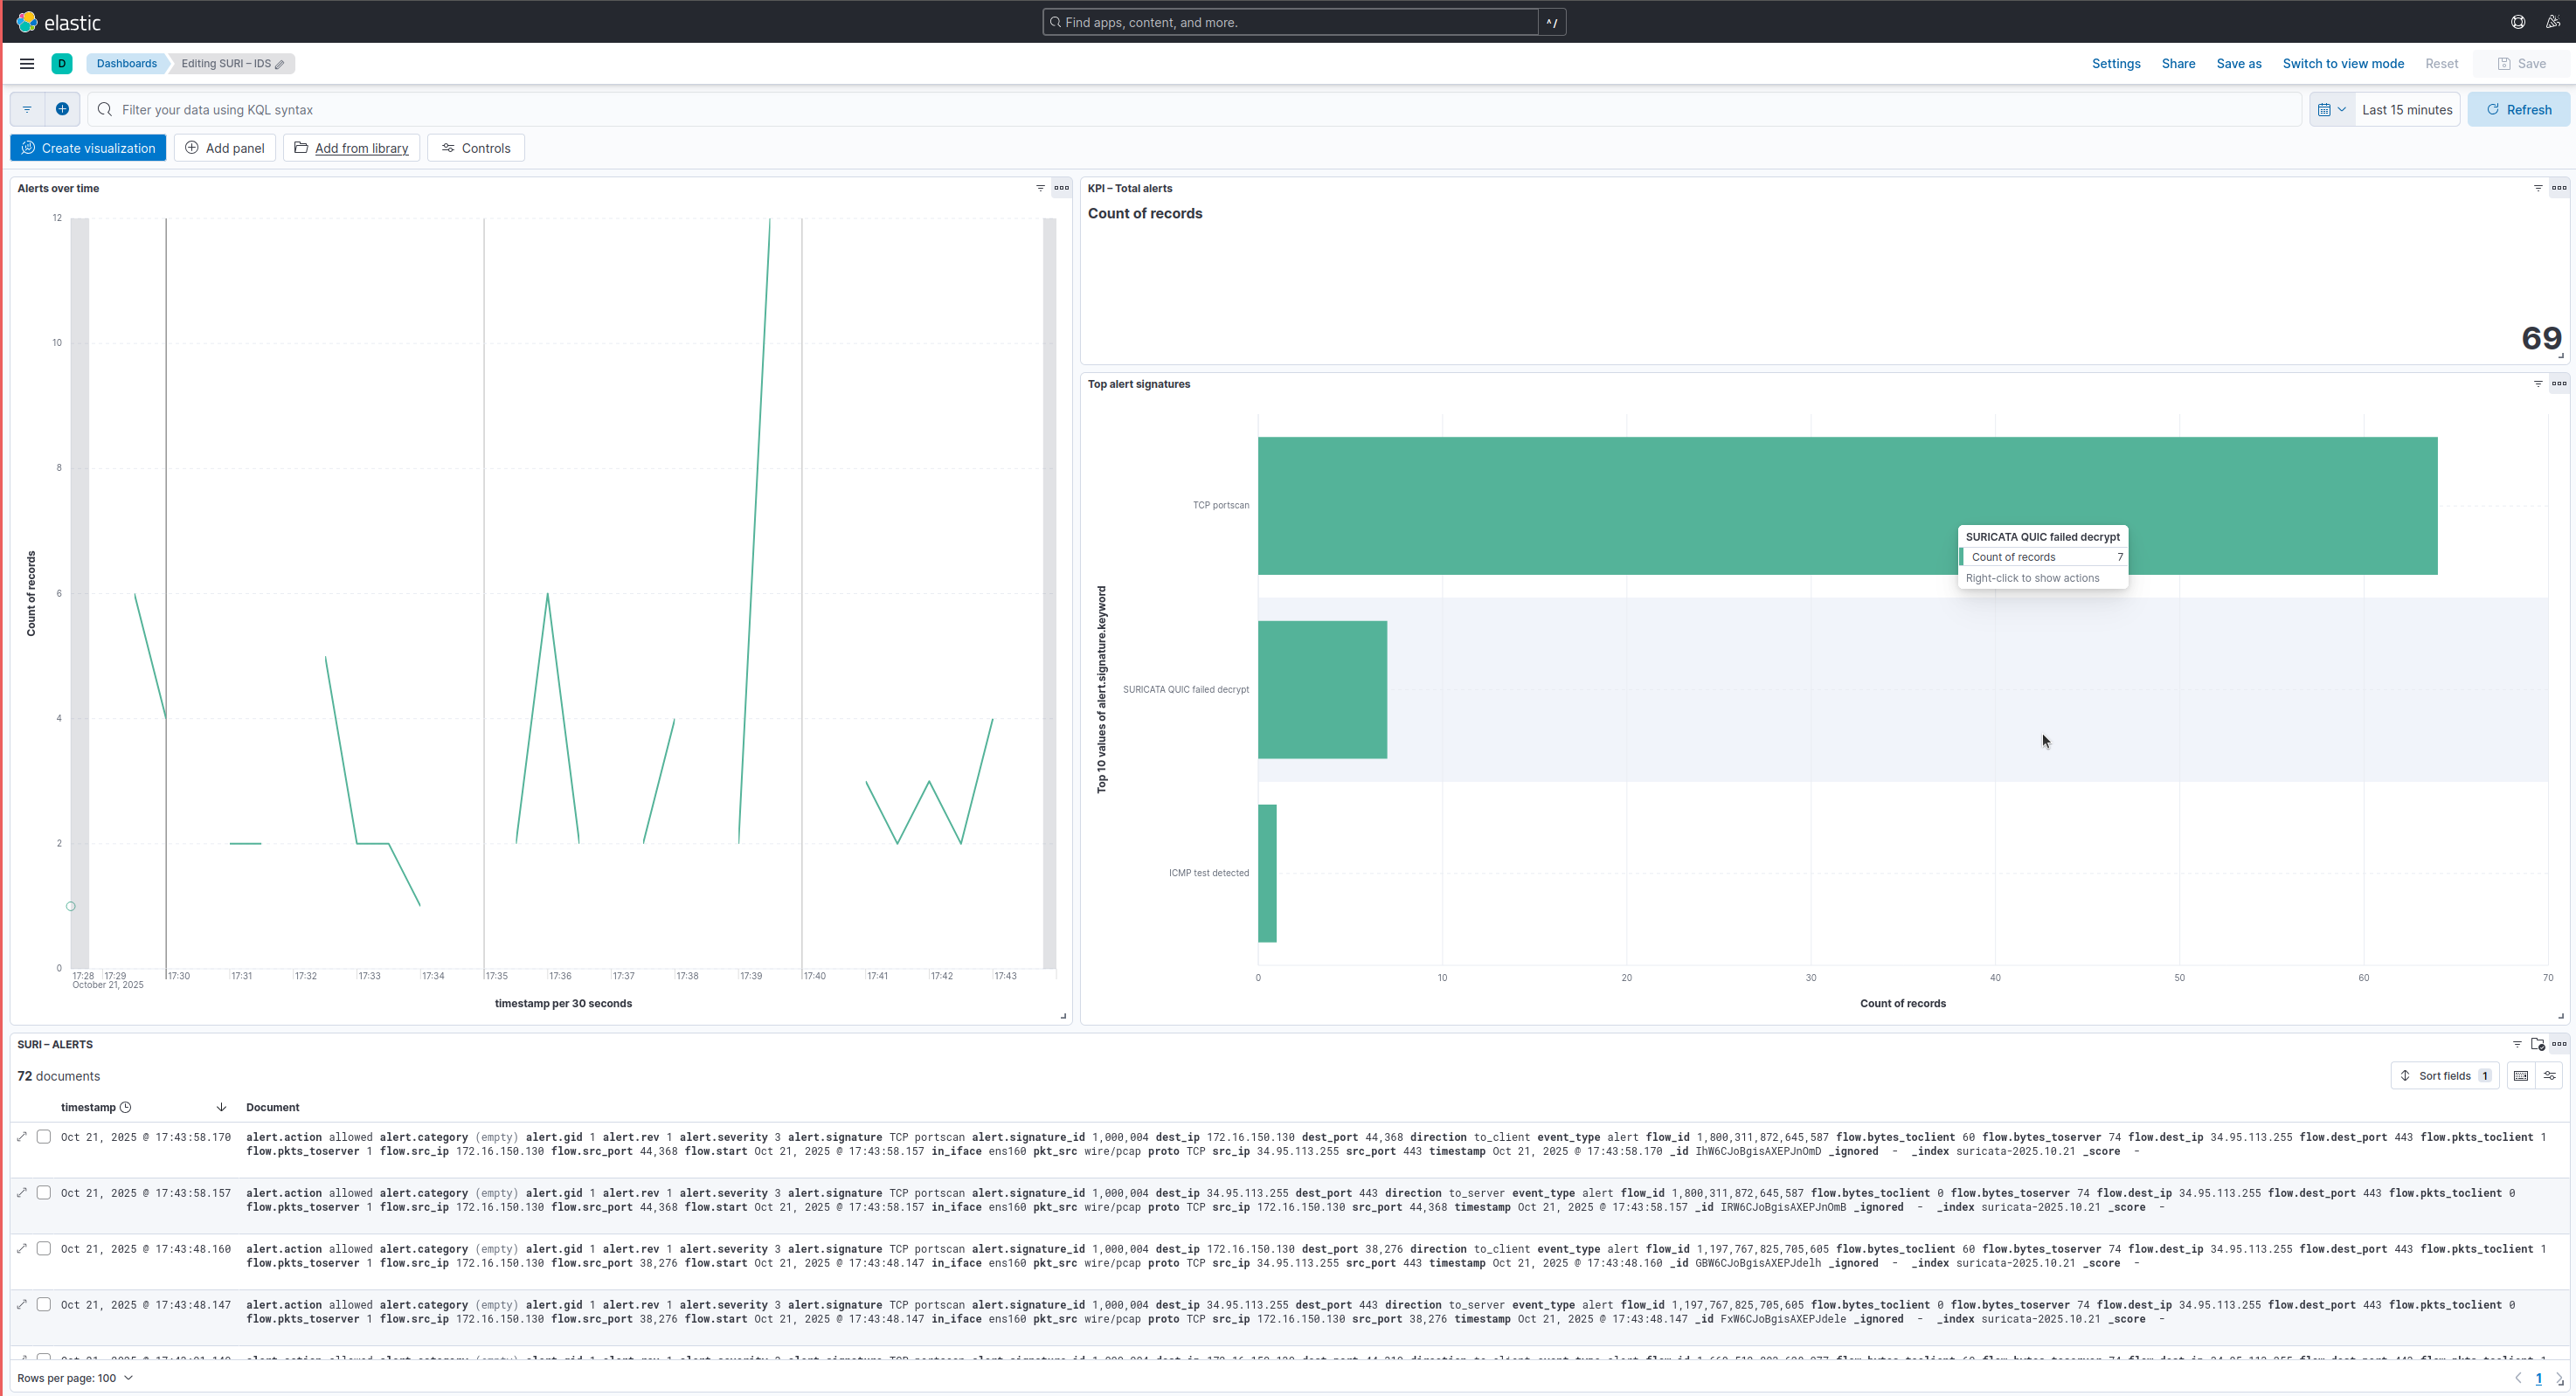
\includegraphics[width=0.6\linewidth]{assets/figures/kibana_dashboard_final.png}
    \caption{Tableau de bord Kibana personnalisé regroupant les visualisations issues des cinq scénarios de détection Suricata.}
    \label{fig:kibana_dashboard_final}
\end{figure}

\clearpage
\section{Point bonus — Automatisation des alertes Slack}

Afin d'améliorer la réactivité du système de détection, un script Python a été mis en place pour envoyer automatiquement les alertes Suricata vers un canal Slack dédié.

Chaque nouvelle alerte écrite dans le fichier \texttt{/var/log/suricata/eve.json} est analysée en temps réel.  
Les informations principales (signature, IP source et destination, niveau de sévérité) sont ensuite transmises via un \textit{webhook} Slack, permettant à l’administrateur d’être notifié instantanément sur mobile ou desktop.

\begin{figure}[H]
    \centering
    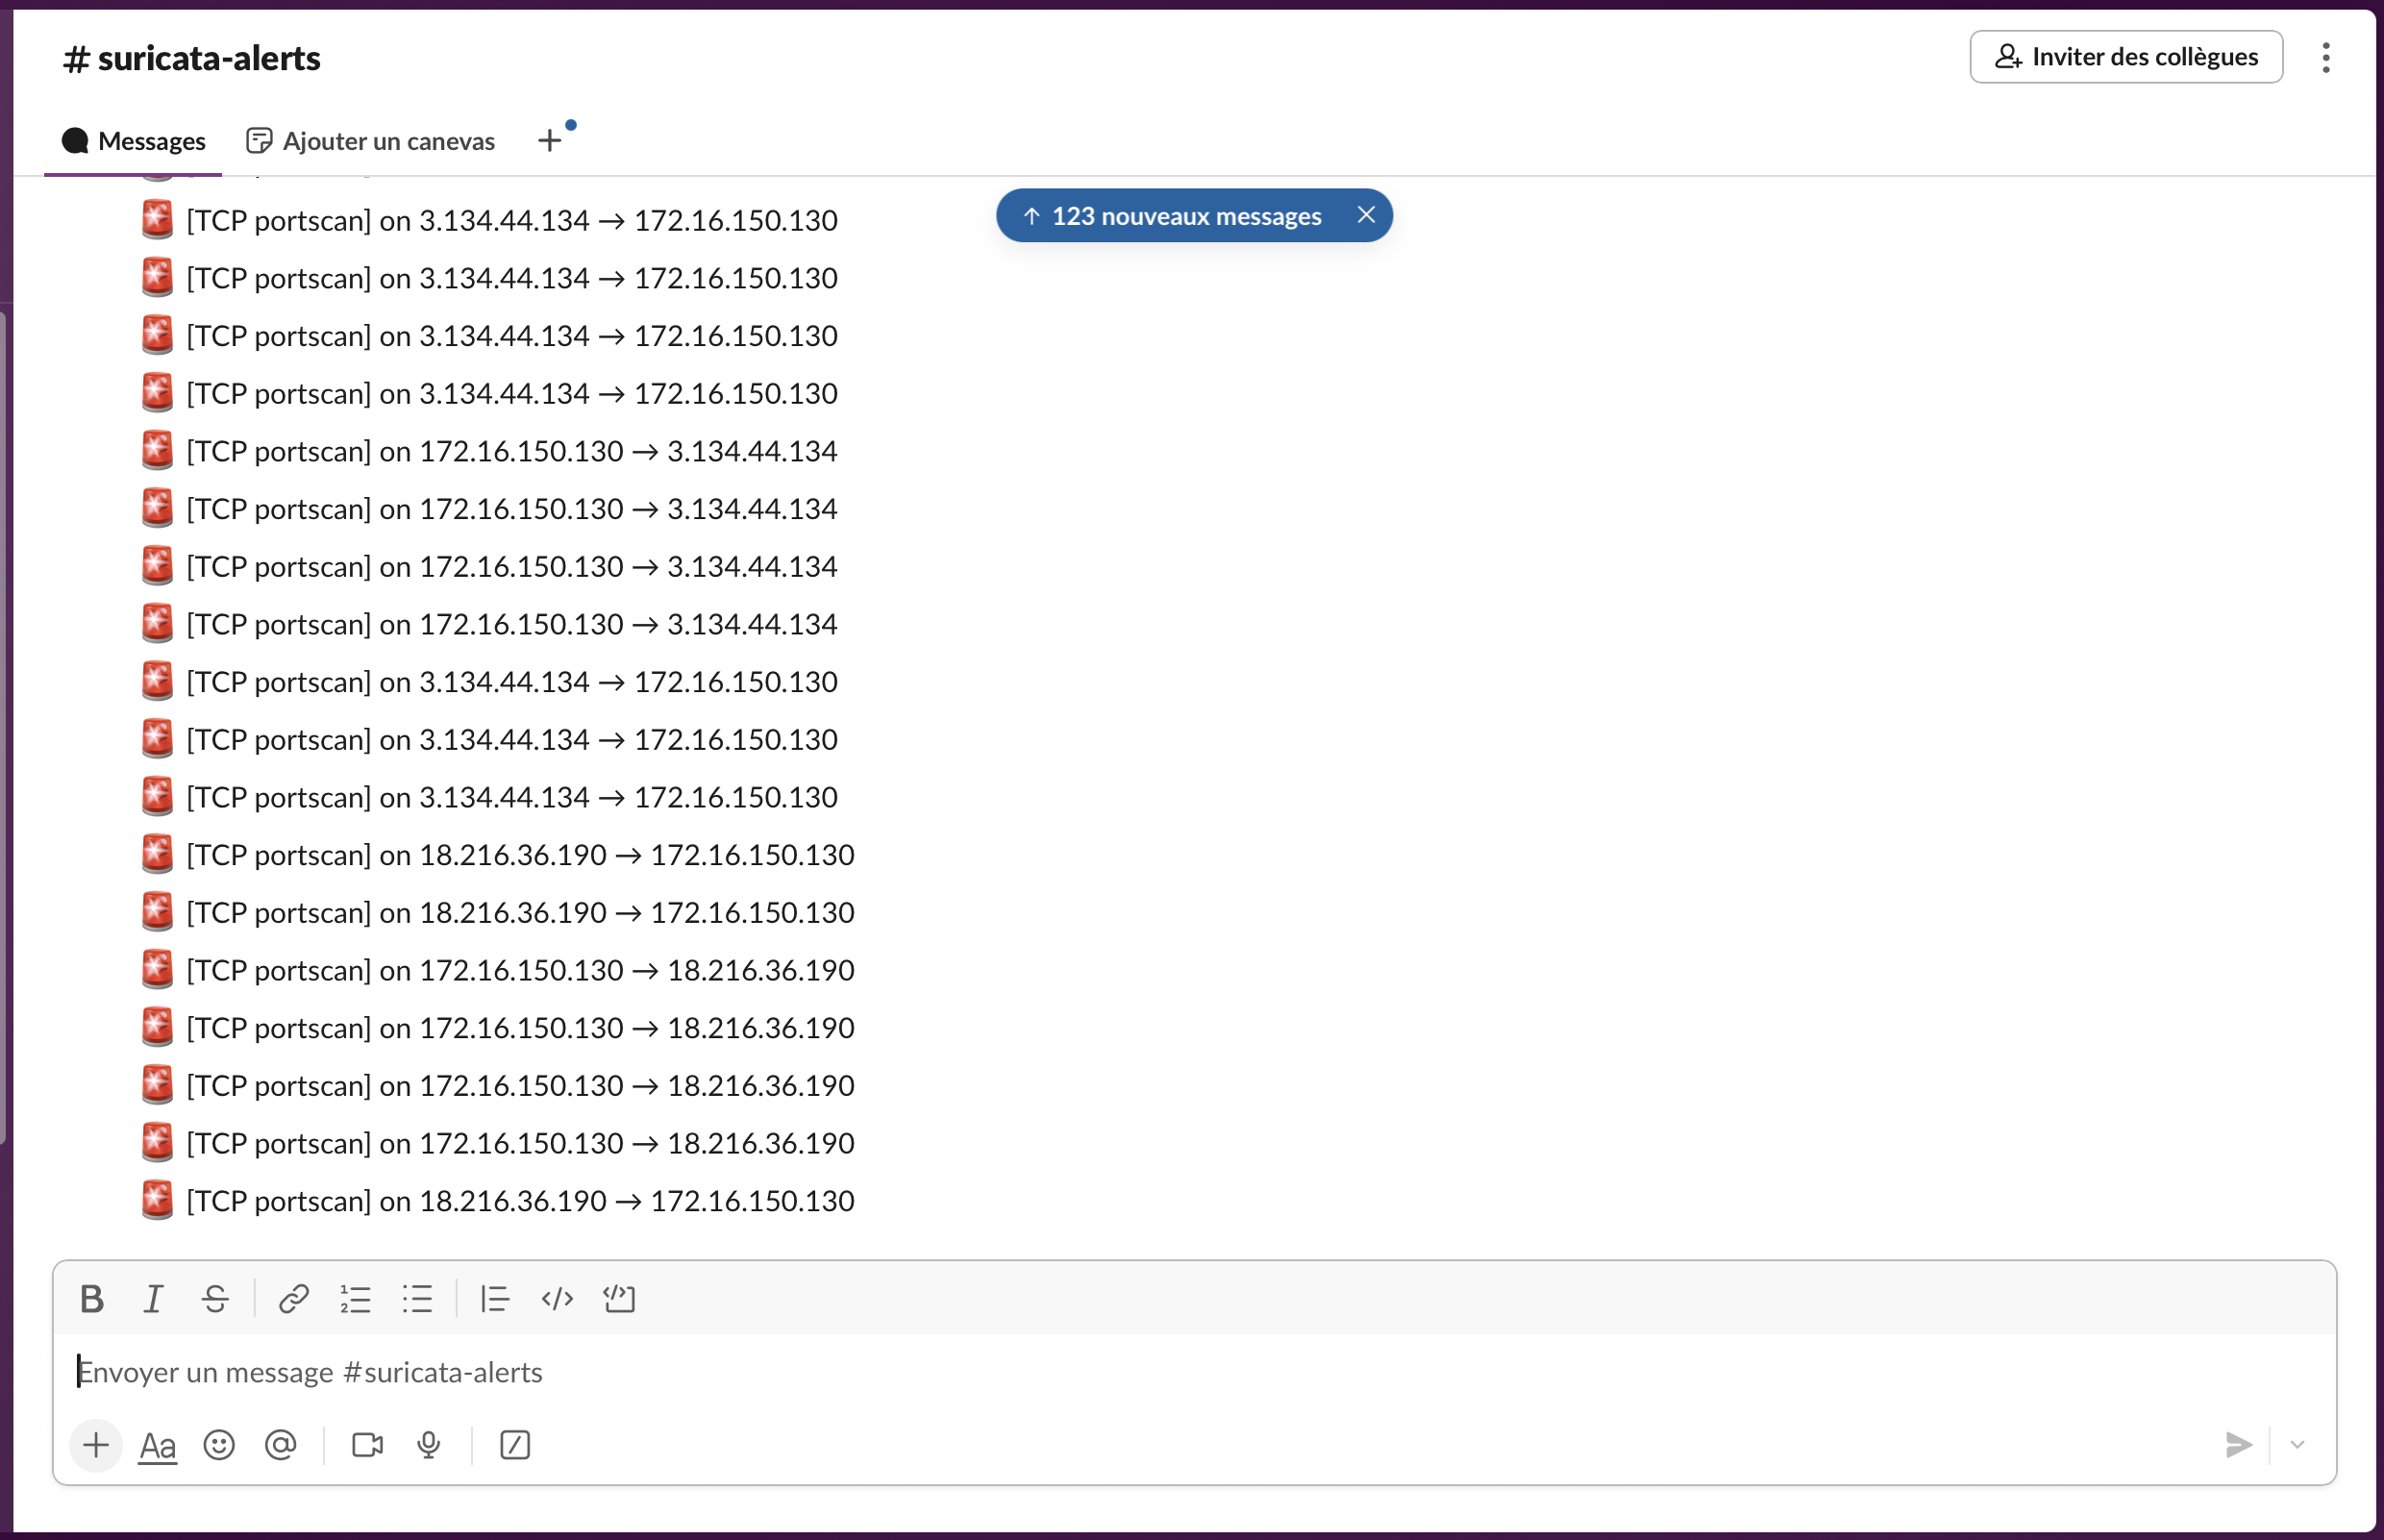
\includegraphics[width=0.9\linewidth]{assets/figures/slack_alert_example.png}
    \caption{Notification automatique d'une alerte Suricata envoyée sur Slack.}
    \label{fig:slack_alert_example}
\end{figure}

Cette automatisation transforme la solution IDS en un véritable outil de supervision active, 
capable de prévenir immédiatement l’administrateur en cas d’incident de sécurité.

\clearpage
\section{Point bonus — Schéma d'architecture (Mermaid)}

La figure~\ref{fig:arch_suricata} présente l’architecture de la solution :
Suricata écoute simultanément sur \texttt{ens160} et \texttt{lo} ; les événements sont écrits dans \texttt{/var/log/suricata/eve.json}, collectés par \texttt{syslog-ng} puis indexés dans \texttt{Elasticsearch}. Les tableaux de bord Kibana exploitent ces données pour l’investigation. Les alertes critiques sont parallèlement envoyées vers Slack via un \textit{webhook}. La rotation des journaux (\texttt{logrotate}) garantit la maîtrise du stockage.

\begin{figure}[H]
  \centering
  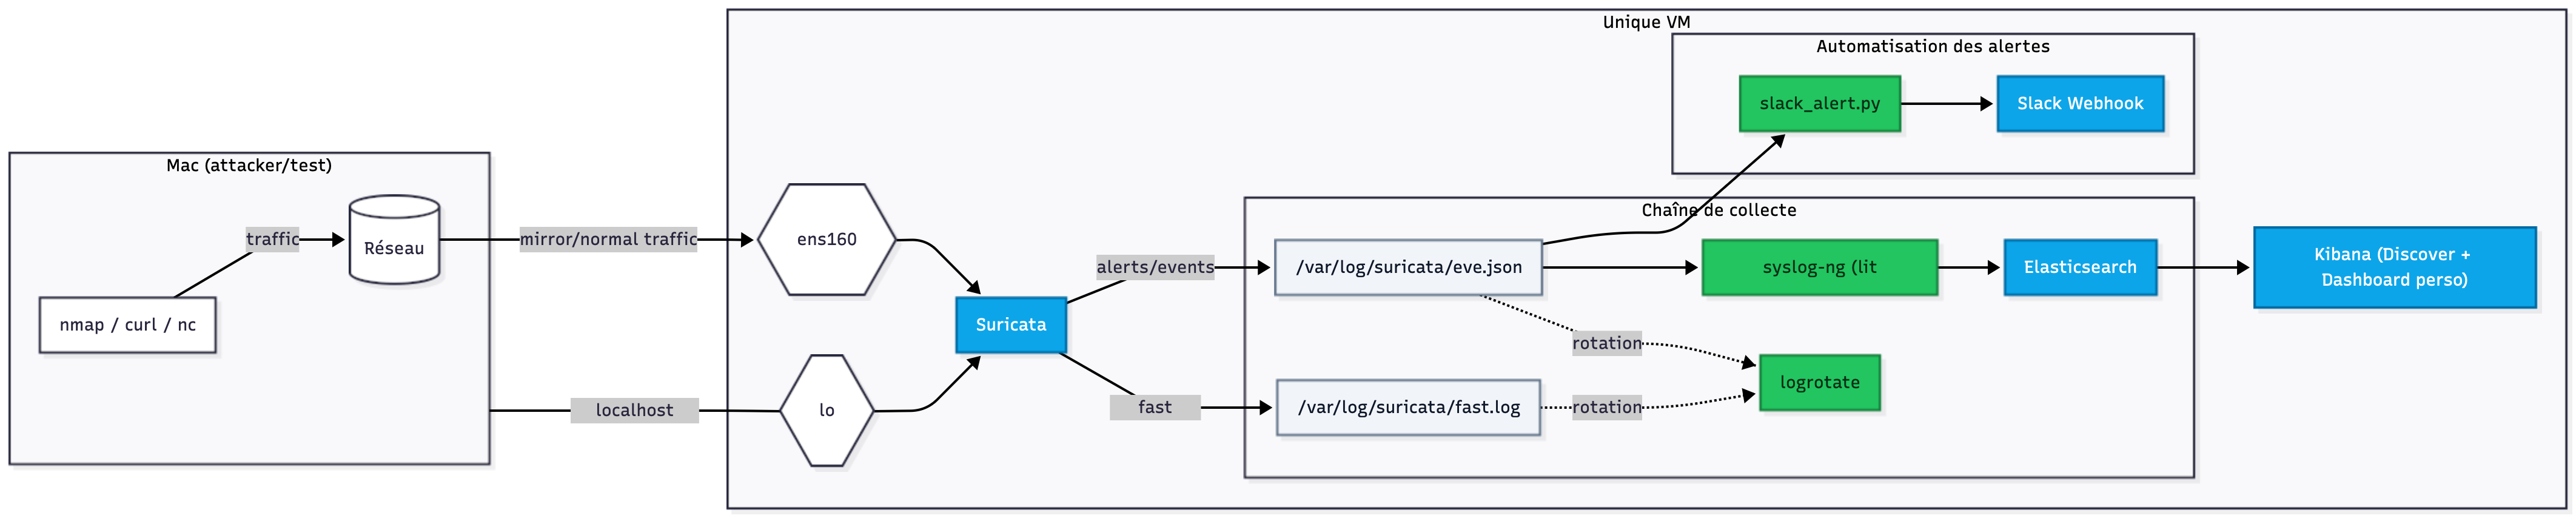
\includegraphics[width=\linewidth]{assets/figures/arch_suricata_stack.png}
  \caption{Chaîne de collecte et supervision : Suricata $\rightarrow$ syslog-ng $\rightarrow$ Elasticsearch $\rightarrow$ Kibana, avec envoi d'alertes Slack et rotation des logs.}
  \label{fig:arch_suricata}
\end{figure}
\chapter{Analyse et discussion}
\label{chap:chap_4}

La principale contrainte du système réside dans la visibilité limitée au niveau du chiffrement, notamment pour les protocoles sécurisés tels que SSH ou HTTPS, dont le contenu reste inaccessible sans inspection TLS.  
De plus, le déploiement sur une unique machine virtuelle limite la scalabilité et ne permet pas de simuler un environnement réseau distribué réel.  
Enfin, l’absence d’une corrélation automatique inter-scénarios ou d’un module d’analyse comportementale réduit la capacité de détection des attaques multi-étapes.

\bigskip
\noindent
Améliorations possibles :  
Une évolution naturelle du projet consisterait à intégrer des outils de réponse et d’automatisation tels que TheHive ou Cortex afin de créer un mini-SOAR (Security Orchestration, Automation and Response).  
L’ajout d’un module de machine learning pour la détection comportementale pourrait également améliorer la précision des alertes et réduire les faux positifs.  
Enfin, la mise en place d’un cluster Elasticsearch distribué et d’un Wazuh Manager offrirait une meilleure résilience et une supervision multi-nœuds.

\bigskip
\noindent
Perspectives et veille technologique :  
Ce projet constitue une base solide pour explorer des approches modernes telles que :
\begin{itemize}
    \item L’intégration d’outils de threat intelligence (MISP, OpenCTI) pour enrichir les alertes avec des indicateurs de compromission connus (IoC) ;
    \item L’adoption d’un pipeline de logs unifié avec Logstash ou Fluentd pour améliorer la normalisation et la performance d’ingestion ;
    \item L’utilisation d’outils de visualisation avancée (Grafana, OpenSearch Dashboards) pour compléter l’analyse de Kibana.
\end{itemize}

\begin{conclusion}

Ce projet a permis de concevoir et de déployer un système complet de détection d’anomalies et de gestion centralisée des journaux de sécurité, basé sur la pile logicielle Suricata, syslog-ng, Elasticsearch, Kibana. 
Grâce à cette architecture, les événements réseau peuvent être détectés, collectés, indexés et visualisés en temps réel au sein d’un tableau de bord unifié, assurant ainsi une traçabilité complète et une meilleure visibilité sur l’activité du réseau.

La configuration de Suricata a permis de mettre en œuvre plusieurs règles de détection locales couvrant différents scénarios d’attaque :  
\textit{ICMP (ping)}, \textit{scan Nmap}, \textit{tentatives SSH}, \textit{fuzzing web} et \textit{accès FTP anonyme}.  
Chacun de ces cas a été validé avec succès, confirmant la capacité du système à identifier ces comportements suspects et ouvrant la voie vers l'identification de bien d'autres attaques, moyennant la mise en place des règles correspondantes dans Suricata.  
Les alertes générées ont ensuite été corrélées et exploitées via Kibana, offrant une visualisation claire et centralisée de l’activité réseau.

En conclusion, ce projet démontre la faisabilité et l’efficacité d’une approche open source pour la détection d’intrusions et la gestion de la sécurité réseau.  

\vspace{3cm}

\begin{figure}[H]
	\centering
	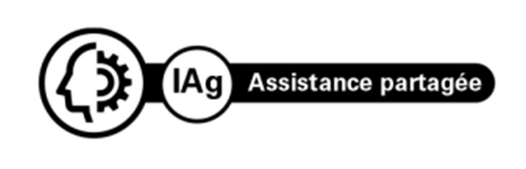
\includegraphics[scale=0.5]{assets/figures/AssistanceIA.png}
	\label{fig:pictoIA}
\end{figure}

\end{conclusion}



%%%%%%%%$%%%%
%%
%% Références
%%
%%%%%%%%%%%%%

%%%%%%%%%%%%%%%%%%%%%%%%%%%%%%%%%%%%%%%%%%%%%%%%%%%%%%%%%%
%%
%% Le fichier BibTeX contenant les références
%% doit se trouver dans le répertoire "assets/references".
%%
%%%%%%%%%%%%%%%%%%%%%%%%%%%%%%%%%%%%%%%%%%%%%%%%%%%%%%%%%%
% \bibliography{assets/references}

%%%%%%%%%%%
%%
%% Annexes
%%
%%%%%%%%%%%
%\appendix

%\include{content/annexe_a}

\end{document}
